% Options for packages loaded elsewhere
\PassOptionsToPackage{unicode}{hyperref}
\PassOptionsToPackage{hyphens}{url}
\documentclass[
]{book}
\usepackage{xcolor}
\usepackage{amsmath,amssymb}
\setcounter{secnumdepth}{5}
\usepackage{iftex}
\ifPDFTeX
  \usepackage[T1]{fontenc}
  \usepackage[utf8]{inputenc}
  \usepackage{textcomp} % provide euro and other symbols
\else % if luatex or xetex
  \usepackage{unicode-math} % this also loads fontspec
  \defaultfontfeatures{Scale=MatchLowercase}
  \defaultfontfeatures[\rmfamily]{Ligatures=TeX,Scale=1}
\fi
\usepackage{lmodern}
\ifPDFTeX\else
  % xetex/luatex font selection
\fi
% Use upquote if available, for straight quotes in verbatim environments
\IfFileExists{upquote.sty}{\usepackage{upquote}}{}
\IfFileExists{microtype.sty}{% use microtype if available
  \usepackage[]{microtype}
  \UseMicrotypeSet[protrusion]{basicmath} % disable protrusion for tt fonts
}{}
\makeatletter
\@ifundefined{KOMAClassName}{% if non-KOMA class
  \IfFileExists{parskip.sty}{%
    \usepackage{parskip}
  }{% else
    \setlength{\parindent}{0pt}
    \setlength{\parskip}{6pt plus 2pt minus 1pt}}
}{% if KOMA class
  \KOMAoptions{parskip=half}}
\makeatother
\usepackage{color}
\usepackage{fancyvrb}
\newcommand{\VerbBar}{|}
\newcommand{\VERB}{\Verb[commandchars=\\\{\}]}
\DefineVerbatimEnvironment{Highlighting}{Verbatim}{commandchars=\\\{\}}
% Add ',fontsize=\small' for more characters per line
\usepackage{framed}
\definecolor{shadecolor}{RGB}{248,248,248}
\newenvironment{Shaded}{\begin{snugshade}}{\end{snugshade}}
\newcommand{\AlertTok}[1]{\textcolor[rgb]{0.94,0.16,0.16}{#1}}
\newcommand{\AnnotationTok}[1]{\textcolor[rgb]{0.56,0.35,0.01}{\textbf{\textit{#1}}}}
\newcommand{\AttributeTok}[1]{\textcolor[rgb]{0.13,0.29,0.53}{#1}}
\newcommand{\BaseNTok}[1]{\textcolor[rgb]{0.00,0.00,0.81}{#1}}
\newcommand{\BuiltInTok}[1]{#1}
\newcommand{\CharTok}[1]{\textcolor[rgb]{0.31,0.60,0.02}{#1}}
\newcommand{\CommentTok}[1]{\textcolor[rgb]{0.56,0.35,0.01}{\textit{#1}}}
\newcommand{\CommentVarTok}[1]{\textcolor[rgb]{0.56,0.35,0.01}{\textbf{\textit{#1}}}}
\newcommand{\ConstantTok}[1]{\textcolor[rgb]{0.56,0.35,0.01}{#1}}
\newcommand{\ControlFlowTok}[1]{\textcolor[rgb]{0.13,0.29,0.53}{\textbf{#1}}}
\newcommand{\DataTypeTok}[1]{\textcolor[rgb]{0.13,0.29,0.53}{#1}}
\newcommand{\DecValTok}[1]{\textcolor[rgb]{0.00,0.00,0.81}{#1}}
\newcommand{\DocumentationTok}[1]{\textcolor[rgb]{0.56,0.35,0.01}{\textbf{\textit{#1}}}}
\newcommand{\ErrorTok}[1]{\textcolor[rgb]{0.64,0.00,0.00}{\textbf{#1}}}
\newcommand{\ExtensionTok}[1]{#1}
\newcommand{\FloatTok}[1]{\textcolor[rgb]{0.00,0.00,0.81}{#1}}
\newcommand{\FunctionTok}[1]{\textcolor[rgb]{0.13,0.29,0.53}{\textbf{#1}}}
\newcommand{\ImportTok}[1]{#1}
\newcommand{\InformationTok}[1]{\textcolor[rgb]{0.56,0.35,0.01}{\textbf{\textit{#1}}}}
\newcommand{\KeywordTok}[1]{\textcolor[rgb]{0.13,0.29,0.53}{\textbf{#1}}}
\newcommand{\NormalTok}[1]{#1}
\newcommand{\OperatorTok}[1]{\textcolor[rgb]{0.81,0.36,0.00}{\textbf{#1}}}
\newcommand{\OtherTok}[1]{\textcolor[rgb]{0.56,0.35,0.01}{#1}}
\newcommand{\PreprocessorTok}[1]{\textcolor[rgb]{0.56,0.35,0.01}{\textit{#1}}}
\newcommand{\RegionMarkerTok}[1]{#1}
\newcommand{\SpecialCharTok}[1]{\textcolor[rgb]{0.81,0.36,0.00}{\textbf{#1}}}
\newcommand{\SpecialStringTok}[1]{\textcolor[rgb]{0.31,0.60,0.02}{#1}}
\newcommand{\StringTok}[1]{\textcolor[rgb]{0.31,0.60,0.02}{#1}}
\newcommand{\VariableTok}[1]{\textcolor[rgb]{0.00,0.00,0.00}{#1}}
\newcommand{\VerbatimStringTok}[1]{\textcolor[rgb]{0.31,0.60,0.02}{#1}}
\newcommand{\WarningTok}[1]{\textcolor[rgb]{0.56,0.35,0.01}{\textbf{\textit{#1}}}}
\usepackage{longtable,booktabs,array}
\usepackage{calc} % for calculating minipage widths
% Correct order of tables after \paragraph or \subparagraph
\usepackage{etoolbox}
\makeatletter
\patchcmd\longtable{\par}{\if@noskipsec\mbox{}\fi\par}{}{}
\makeatother
% Allow footnotes in longtable head/foot
\IfFileExists{footnotehyper.sty}{\usepackage{footnotehyper}}{\usepackage{footnote}}
\makesavenoteenv{longtable}
\usepackage{graphicx}
\makeatletter
\newsavebox\pandoc@box
\newcommand*\pandocbounded[1]{% scales image to fit in text height/width
  \sbox\pandoc@box{#1}%
  \Gscale@div\@tempa{\textheight}{\dimexpr\ht\pandoc@box+\dp\pandoc@box\relax}%
  \Gscale@div\@tempb{\linewidth}{\wd\pandoc@box}%
  \ifdim\@tempb\p@<\@tempa\p@\let\@tempa\@tempb\fi% select the smaller of both
  \ifdim\@tempa\p@<\p@\scalebox{\@tempa}{\usebox\pandoc@box}%
  \else\usebox{\pandoc@box}%
  \fi%
}
% Set default figure placement to htbp
\def\fps@figure{htbp}
\makeatother
\setlength{\emergencystretch}{3em} % prevent overfull lines
\providecommand{\tightlist}{%
  \setlength{\itemsep}{0pt}\setlength{\parskip}{0pt}}
\usepackage[]{natbib}
\bibliographystyle{plainnat}
\usepackage{booktabs}
\usepackage{booktabs}
\usepackage{longtable}
\usepackage{array}
\usepackage{multirow}
\usepackage{wrapfig}
\usepackage{float}
\usepackage{colortbl}
\usepackage{pdflscape}
\usepackage{tabu}
\usepackage{threeparttable}
\usepackage{threeparttablex}
\usepackage[normalem]{ulem}
\usepackage{makecell}
\usepackage{xcolor}
\usepackage{bookmark}
\IfFileExists{xurl.sty}{\usepackage{xurl}}{} % add URL line breaks if available
\urlstyle{same}
\hypersetup{
  pdftitle={Lie Groups and Lie Algbera},
  pdfauthor={Ashan De Silva (Student Number: 008058631)},
  hidelinks,
  pdfcreator={LaTeX via pandoc}}

\title{Lie Groups and Lie Algbera}
\author{Ashan De Silva (Student Number: 008058631)}
\date{2026-01-03}

\usepackage{amsthm}
\newtheorem{theorem}{Theorem}[chapter]
\newtheorem{lemma}{Lemma}[chapter]
\newtheorem{corollary}{Corollary}[chapter]
\newtheorem{proposition}{Proposition}[chapter]
\newtheorem{conjecture}{Conjecture}[chapter]
\theoremstyle{definition}
\newtheorem{definition}{Definition}[chapter]
\theoremstyle{definition}
\newtheorem{example}{Example}[chapter]
\theoremstyle{definition}
\newtheorem{exercise}{Exercise}[chapter]
\theoremstyle{definition}
\newtheorem{hypothesis}{Hypothesis}[chapter]
\theoremstyle{remark}
\newtheorem*{remark}{Remark}
\newtheorem*{solution}{Solution}
\begin{document}
\maketitle

{
\setcounter{tocdepth}{1}
\tableofcontents
}
\chapter{Introduction}\label{introduction}

Physical systems often show continuous symmetries, such as rotational symmetry or Lorentz symmetry. These symmetries form what mathematicians call \textbf{Lie groups}. A Lie group is a smooth manifold that also has a group structure. This means it combines geometry with algebraic operations. To make the study of these curved structures easier, we look at the associated \textbf{Lie algebra}. The Lie algebra is defined as the tangent space at the identity element of the group.

Because the Lie algebra is a linear vector space, it is much easier to perform calculations with it than with the full group. Even though it is simpler, it still carries the local properties of the group through a tool called the \textbf{matrix exponential map}.

In quantum mechanics, symmetries are described by unitary operators acting on the Hilbert space of a system. When the Hamiltonian of the system commutes with these symmetry operators, the energy states stay the same under the symmetry. This principle is very important for solving problems, such as finding the energy levels of the hydrogen atom.

This project focuses on \textbf{matrix Lie groups}, which are closed subgroups of the general linear group \(GL(n; \mathbb{C})\). We will study how the way a group behaves leads to the way its algebra behaves. In the algebra, the group operation is replaced by a bracket operation, defined as \([X,Y] = XY - YX\).

A very important detail in this study is the idea of \textbf{projective representations}. These are used because in quantum mechanics, two states are physically the same if they only differ by a phase factor. For groups that are not simply connected, like the rotation group \(SO(3)\), some representations of the algebra do not match the group perfectly. Instead, they match a related group called the universal cover. For example, the simply connected group \(SU(2)\) is used as the cover for \(SO(3)\) to correctly describe particle spin in quantum mechanics.

\section{Notation and Some definitions}\label{notation-and-some-definitions}

\begin{enumerate}
\def\labelenumi{\arabic{enumi}.}
\tightlist
\item
  \(\mathrm{GL}_n(\mathbb{C})\): the group of all \(n \times n\) invertible matrices with entries in the field \(\mathbb{F}\).
\item
  \(M_n(\mathbb{C})\): the set of all \(n \times n\) matrices with entries in the field \(\mathbb{F}\).
\item
  \(U(n)\): \(n \times n\) unitary group
\item
  \(SU\): Special Unitary Group (Unitary Group + det=1)
\item
  \(O(n)\): \(n \times n\) Orthogonal group
\item
  \(SO(n)\): \(n \times n\) Special orthogonal Group (Orthogonal Group + det=1)
\end{enumerate}

\chapter{Lie Groups}\label{lie-groups}

\begin{definition}[Lie Group]
\protect\hypertarget{def:unnamed-chunk-1}{}\label{def:unnamed-chunk-1}A \emph{Lie group} is a smooth manifold \(G\) which is also a group, such that the group multiplication
\[\mu: G \times G \to G, \quad (g,h) \mapsto gh\]
and the inverse map
\[\iota: G \to G, \quad g \mapsto g^{-1}\]
are both smooth.
\end{definition}

\begin{example}
\protect\hypertarget{exm:unnamed-chunk-2}{}\label{exm:unnamed-chunk-2}Let \(G = \mathbb{R} \times \mathbb{R} \times S\), equipped with the group operation
\[(x_1, y_1, \lambda_1) \cdot (x_2, y_2, \lambda_2) = (x_1 + x_2,\, y_1 + y_2,\, e^{ix_1y_2}\lambda_1 \lambda_2). \text{ and } \]
\[(x,y,\lambda)^{-1}=\left(-x,\; -y,\; e^{ixy}\lambda^{-1}\right)\]\$\$
Then \(G\) is a Lie group.
\end{example}

\begin{definition}
\protect\hypertarget{def:unnamed-chunk-3}{}\label{def:unnamed-chunk-3}Let \(A_m\) be a sequence of complex matrices in \(\mathbb{M}_n(\mathbb{C})\). We say that \(A_m \to A\) (i.e., \(A_m\) converges to a matrix \(A\)) if each entry of \(A_m\) converges to the corresponding entry of \(A\) as \(m \to \infty\); In other words,
\[(A_m)_{jk} \to A_{jk} \quad \text{for all } 1 \leq j, k \leq n.\]
\end{definition}

\begin{definition}[Matrix Lie Group]
\protect\hypertarget{def:unnamed-chunk-4}{}\label{def:unnamed-chunk-4}A \emph{matrix Lie group} is a subgroup \(G \subseteq \mathrm{GL}(n, \mathbb{C})\) with the following property: If \(\{A_m\}\) is any sequence of matrices in \(G\) such that \(A_m \to A\), then either \(A \in G\) or \(A\) is not invertible.
\end{definition}

\begin{example}[Example of Matrix Linear Groups]
\protect\hypertarget{exm:unnamed-chunk-5}{}\label{exm:unnamed-chunk-5}\leavevmode

\begin{enumerate}
\def\labelenumi{\arabic{enumi}.}
\tightlist
\item
  General Linear Groups over \(\mathbb{C}\) and \(\mathbb{R}\).
\end{enumerate}

\begin{itemize}
\tightlist
\item
  \(GL_n(\mathbb{C})\) is sub group itsself.
\item
  if \(A_m\) is a sequence of matrices in \(GL_n(\mathbb{C}\) and \(A_m\) converges to \(A\), then by the definition of \(GL_n(\mathbb{C}\), either \(A\) is in \(GL_n(\mathbb{C}\),or \(A\) is not invertible.
\end{itemize}

\begin{enumerate}
\def\labelenumi{\arabic{enumi}.}
\tightlist
\item
  Special linear Groups over \(\mathbb{C}\) and \(\mathbb{R}\).
\item
\end{enumerate}

\end{example}

\begin{example}[Non example]
\protect\hypertarget{exm:unnamed-chunk-6}{}\label{exm:unnamed-chunk-6}Let \(\alpha \in \mathbb{R} \setminus \mathbb{Q}\), and define the subgroup \(G \subseteq \mathrm{GL}(2, \mathbb{C})\) consisting of matrices of the form

\[G = \left\{
\begin{pmatrix}
e^{it} & 0 \\
0 & e^{i\alpha t}
\end{pmatrix}
: t \in \mathbb{R}
\right\}.\]

Clearly, \(G\) is a subgroup of \(\mathrm{GL}(2, \mathbb{C})\). The closure of \(G\) in the standard topology is the torus subgroup

\[\overline{G} = \left\{
\begin{pmatrix}
e^{i\theta} & 0 \\
0 & e^{i\phi}
\end{pmatrix}
: \theta, \phi \in \mathbb{R}
\right\}
= \left\{
\begin{pmatrix}
z_1 & 0 \\
0 & z_2
\end{pmatrix}
: |z_1| = |z_2| = 1
\right\},\]

which is a compact Lie group. Since \(G\) is not closed, it fails the closure condition required for matrix Lie groups. Thus, \(G\) is not a matrix Lie group.

This subgroup \(G\) is sometimes referred to as an \emph{irrational line in a torus}.
\end{example}

I had problem synchronized with yellow dots. Sorry about that.

--\pandocbounded{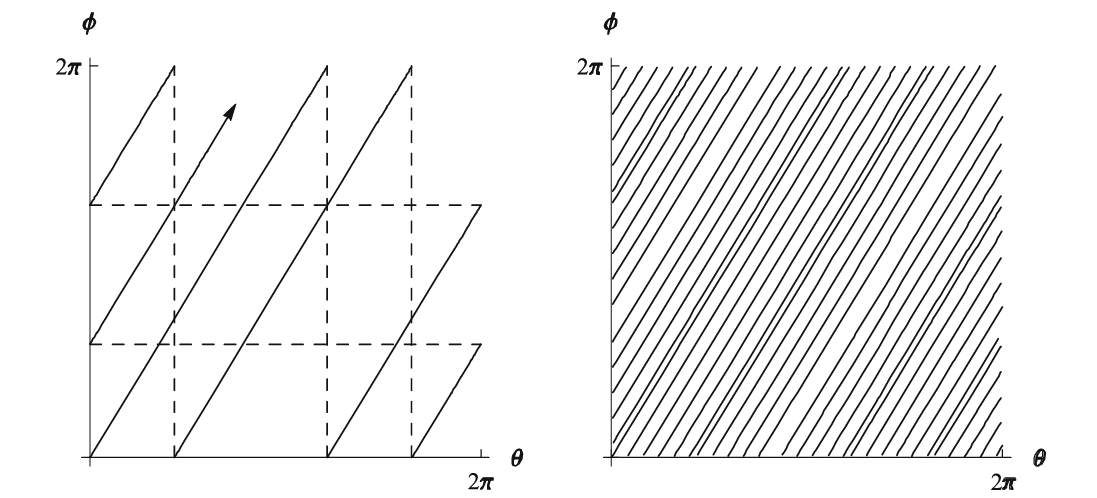
\includegraphics[keepaspectratio]{image.png}}

\begin{definition}[Lie Group homomorphism and Isomorphisms]
\protect\hypertarget{def:unnamed-chunk-8}{}\label{def:unnamed-chunk-8}Let \(G\) and \(H\) be matrix Lie groups. A map \(\varphi : G \to H\) is called a \emph{Lie group homomorphism} if

\begin{enumerate}
\def\labelenumi{\roman{enumi}.}
\tightlist
\item
  \(\varphi\) is a group homomorphism, and
\item
  \(\varphi\) is continuous.
\end{enumerate}

If, in addition, \(\varphi\) is one-to-one and onto, and the inverse map \(\varphi^{-1}\) is continuous, then \(\varphi\) is called a \emph{Lie group isomorphism}.
\end{definition}

\begin{example}[Examples of Lie Group Homomorphisms]
\protect\hypertarget{exm:unnamed-chunk-9}{}\label{exm:unnamed-chunk-9}\leavevmode

\begin{enumerate}
\def\labelenumi{\arabic{enumi}.}
\item
  The determinant is a homomorphism \(\det : \mathrm{GL}_n(\mathbb{C}) \to \mathbb{C}\setminus \{0\}\)
\item
  The map \(\varphi : \mathbb{R} \to \mathrm{SO}(2)\), defined by
  \[\varphi(t) = \begin{pmatrix} \cos t & -\sin t \\ \sin t & \cos t \end{pmatrix}\]
  is also a group homomorphism.
\end{enumerate}

\end{example}

\chapter{Lie Algebra}\label{lie-algebra}

\begin{definition}[Lie Algebra]
\protect\hypertarget{def:unnamed-chunk-10}{}\label{def:unnamed-chunk-10}Let \(\mathbb{F}\) be a field. A \emph{Lie algebra} over \(\mathbb{F}\) is a vector space \(\mathfrak{g}\) over \(\mathbb{F}\) together with a map \([\cdot,\cdot] : \mathfrak{g} \times \mathfrak{g} \to \mathfrak{g}\), called the \emph{Lie bracket}, satisfying the following properties:

\begin{enumerate}
\def\labelenumi{\arabic{enumi}.}
\item
  \textbf{Bi-linearity:} The bracket \([\cdot,\cdot]\) is bilinear.
\item
  \textbf{Skew-symmetry:} For all \(X,Y \in \mathfrak{g}\),
  \[[X,Y] = -[Y,X].\]
\item
  \textbf{Jacobi identity:} For all \(X,Y,Z \in \mathfrak{g}\),
  \[[X,[Y,Z]] + [Y,[Z,X]] + [Z,[X,Y]] = 0.\]
\end{enumerate}

Two elements \(X,Y \in \mathfrak{g}\) are said to \emph{commute} if \([X,Y] = 0\). The Lie algebra \(\mathfrak{g}\) is called \emph{commutative} (or \emph{abelian}) if \([X,Y] = 0\) for all \(X,Y \in \mathfrak{g}\).
\end{definition}

\begin{example}
\protect\hypertarget{exm:unnamed-chunk-11}{}\label{exm:unnamed-chunk-11}Let \(\mathfrak{g} = \mathbb{R}^3\) and define the bracket
\[[x,y] = x \times y, \quad x,y \in \mathbb{R}^3,\]
where \(x \times y\) denotes the cross product. Then \(\mathfrak{g}\) is a Lie algebra.
\end{example}

\begin{proof}
Bilinearity and skew-symmetry are standard properties of the cross product. To verify the Jacobi identity, it suffices (by bilinearity) to check it when
\[x = e_j, \quad y = e_k, \quad z = e_\ell,\]
where \(e_1, e_2, e_3\) are the standard basis vectors of \(\mathbb{R}^3\).

\begin{itemize}
\tightlist
\item
  If \(j,k,\ell\) are all equal, each term in the Jacobi identity is zero.
\item
  If \(j,k,\ell\) are all distinct, the cross product of any two of \(e_j, e_k, e_\ell\) is a multiple of the third, so again each term in the Jacobi identity is zero.
\item
  It remains to consider the case in which two of \(j,k,\ell\) are equal and the third is different. By reordering the terms in the Jacobi identity as necessary, it suffices to verify
  \[[e_j,[e_j,e_k]] + [e_j,[e_k,e_j]] + [e_k,[e_j,e_j]] = 0. \qquad (3.1)\]
\end{itemize}

The first two terms in (3.1) are negatives of each other, and the third is zero.

Thus the Jacobi identity holds, and \(\mathfrak{g}\) is a Lie algebra.
\end{proof}

\begin{example}
\protect\hypertarget{exm:unnamed-chunk-13}{}\label{exm:unnamed-chunk-13}Let \(A\) be an associative algebra and let \(\mathfrak{g}\) be a subspace of \(A\) such that
\[XY - YX \in \mathfrak{g} \quad \text{for all } X,Y \in \mathfrak{g}.\]

Then \(\mathfrak{g}\) is a Lie algebra with bracket operation defined by
\[[X,Y] = XY - YX.\]
\end{example}

\begin{proof}
It is very easy to show the bilinear and skew symmetry properties. So, just go for Jacobi Identity.

Let \(X,Y,Z \in \mathfrak{g}\), consider

\begin{align*}
[X,[Y,Z]] &= X(YZ - ZY) - (YZ - ZY)X = XYZ - XZY - YZX + ZYX,\\
[Y,[Z,X]] &= Y(ZX - XZ) - (ZX - XZ)Y = YZX - YXZ - ZXY + XZY,\\
[Z,[X,Y]] &= Z(XY - YX) - (XY - YX)Z = ZXY - ZYX - XYZ + YXZ.
\end{align*}

Adding these three expressions together, every monomial in \(X,Y,Z\) appears exactly twice, once with a plus sign and once with a minus sign:

\begin{align*}
(XYZ - XYZ) + (XZY - XZY) + (YZX - YZX) + (YXZ - YXZ) \\+ (ZXY - ZXY) + (ZYX - ZYX) = 0.
\end{align*}
\end{proof}

\chapter{Matrix Exponential}\label{matrix-exponential}

The exponential of a matrix plays a crucial role in the theory of Lie groups. The exponential enters into the definition of the Lie algebra of a matrix Lie group and is the mechanism for passing information from the Lie algebra to the Lie group.

\begin{definition}[Matrix Exponential]
\protect\hypertarget{def:mat_exp}{}\label{def:mat_exp}If \(X\) is an \(n \times n\) matrix, we define the exponential of \(X\), denoted \(e^X\) or \(\exp(X)\), by the usual power series
\begin{equation}
e^X = \sum_{m=0}^{\infty} \frac{X^m}{m!},\label{eq:matrixexp}
\end{equation}
where \(X^0=I\), and \(X^m\) denotes the repeated matrix product of \(X\) with itself.
\end{definition}

\begin{proposition}
\protect\hypertarget{prp:unnamed-chunk-15}{}\label{prp:unnamed-chunk-15}The series \eqref{eq:matrixexp} converges for all \(X \in M_n(\mathbb{C})\), and \(e^X\) is a continuous function of \(X\).
\end{proposition}

\begin{theorem}
\protect\hypertarget{thm:thm1}{}\label{thm:thm1}

Let \(X,Y \in M_n(\mathbb{C})\). Then the following properties hold:

\begin{enumerate}
\def\labelenumi{\arabic{enumi}.}
\tightlist
\item
  \(e^{0} = I\)
\item
  \((e^{X})^{\mathrm{T}} = e^{X^{\mathrm{T}}}\qquad\text{and}\qquad(e^{X})^{*} = e^{X^{*}}\)
\item
  If \(A\) is an invertible \(n \times n\) matrix, then\\
  \(e^{AXA^{-1}} = A\, e^{X}\, A^{-1}\)
\item
  \(\det(e^{X}) = e^{\operatorname{trace}(X)}\)
\item
  If \(XY = YX\), then \(e^{X+Y} = e^{X} e^{Y}\)
\item
  \(e^{X} \text{ is invertible and } (e^{X})^{-1} = e^{-X}\)
\item
  Even if \(XY \neq YX\), we have \(e^{X+Y} = \lim_{m\to\infty} \left(e^{X/m} e^{Y/m}\right)^{m}\) (This is a special case of the \textbf{Trotter Product Formula}.)
\end{enumerate}

\end{theorem}

\begin{proof}
\leavevmode

\begin{enumerate}
\def\labelenumi{\arabic{enumi}.}
\tightlist
\item
  It is trivial from the defnition @ref(def:mat\_exp).
\item
  This is follows by taking term-by-term adjoints in the series for \(e^X\).
\item
  This is also easily verified using term-by-term computation.
\item
  On schur decomposition, Over \(\mathbb{C}\), any matrix \(X\) is similar to an upper triangular matrix \(T\). That is, there exists an invertible matrix \(S\) such that, (X=STS\^{}\{-1\}), where \(T\) is upper triangular. By proptery 3,
  \[
  e^X = e^{STS^{-1}}= Se^TS^{-1}
  \]
  Then,\[\det(e^X)=\det(Se^TS^{-1})=\det(e^T).\]
  For the trace,
  \[\operatorname{tr}(X)=\operatorname{tr}(STS^{-1})=\operatorname{tr}(T).\]
  Furthur we can calualate
\end{enumerate}

\[
\det(e^{T}) = \prod_{i=1}^{n} e^{\lambda_i}
= e^{\lambda_1} e^{\lambda_2} \cdots e^{\lambda_n}
= e^{\lambda_1 + \lambda_2 + \cdots + \lambda_n}
= e^{\operatorname{tr}(T)}.
\]

By some computaiaonal,\(e^{T}\) is upper triangular with diagonal entries \(e^{\lambda_1}, \dots, e^{\lambda_n}\). Thus, \(\det(e^X)=\det(e^T)\).

Now combining all the results,
\[
\det(e^{X}) = \det(e^{T}) = e^{\operatorname{tr}(T)} = e^{\operatorname{tr}(X)}.
\]

\begin{enumerate}
\def\labelenumi{\arabic{enumi}.}
\setcounter{enumi}{4}
\tightlist
\item
  First, note that both series both series \(e^X\) and \(e^Y\) converge absolutely. So, we can multiply them term by term,
  \begin{equation}
  e^X e^Y = \sum_{m=0}^{\infty} \sum_{k=0}^{m} \frac{X^k}{k!} \frac{Y^{\,m-k}}{(m-k)!}
  = \sum_{m=0}^{\infty} \frac{1}{m!} \sum_{k=0}^{m} \binom{m}{k} X^k Y^{\,m-k}. \label{eq:exp25}
  \end{equation}
  If \(X\) and \(Y\) commute, then
  \[(X+Y)^m = \sum_{k=0}^{m} \binom{m}{k} X^k Y^{\,m-k},\]
  so \eqref{eq:exp25} becomes
  \[e^X e^Y = \sum_{m=0}^{\infty} \frac{(X+Y)^m}{m!} = e^{X+Y}.\]
\item
  This is foolowed from Property 5 by taking Y = −X and applying Property.
\item
  Proof is ommited. (Becasue it is quite long.)
\end{enumerate}

\end{proof}

\section{Computing Exponential}\label{computing-exponential}

If \(X\) is diagonalizable, then there exist invertible \(A\) and \(\lambda_1,...,\lambda_n\) such that

\[X = A
\begin{bmatrix}
{\lambda_1} & 0 & \cdots & 0 \\
0 & {\lambda_2} & \cdots & 0 \\
\vdots & \vdots & \ddots & \vdots \\
0 & 0 & \cdots & {\lambda_n}
\end{bmatrix}
A^{-1}\]

Then by Theorem \ref{thm:thm1} fourth property, we get the following:

\[e^X = A
\begin{bmatrix}
e^{\lambda_1} & 0 & \cdots & 0 \\
0 & e^{\lambda_2} & \cdots & 0 \\
\vdots & \vdots & \ddots & \vdots \\
0 & 0 & \cdots & e^{\lambda_n}
\end{bmatrix}A^{-1}\]

If \(X\) is nilpotent then the series that defines \(e^X\) terminates.

\begin{example}
\protect\hypertarget{exm:unnamed-chunk-17}{}\label{exm:unnamed-chunk-17}Consider the matrices

\[X_1 =
\begin{bmatrix}
0 & -a \\
a & 0
\end{bmatrix}, \quad
X_2 =
\begin{bmatrix}
0 & a & b \\
0 & 0 & c \\
0 & 0 & 0
\end{bmatrix}, \quad
X_3 =
\begin{bmatrix}
a & b \\
0 & a
\end{bmatrix}.\]

Then

\[e^{X_1} =
\begin{bmatrix}
\cos a & -\sin a \\
\sin a & \cos a
\end{bmatrix}, \text{ and }
e^{X_2} =
\begin{bmatrix}
1 & a & b + \tfrac{ac}{2} \\
0 & 1 & c \\
0 & 0 & 1
\end{bmatrix}, \text{ and } 
e^{X_3} =
\begin{bmatrix}
e^a & e^a b \\
0 & e^a
\end{bmatrix}.\]
\end{example}

\begin{proof}
\[e^{X_1} = 
\begin{bmatrix} 1 & i \\ i & 1 \end{bmatrix}
\begin{bmatrix} e^{-ia} & 0 \\ 0 & e^{ia} \end{bmatrix}
\frac{1}{2}
\begin{bmatrix} 1 & -i \\ -i & 1 \end{bmatrix}.\]
\end{proof}

\chapter{The Lie Algebra of a Matrix Lie Group}\label{the-lie-algebra-of-a-matrix-lie-group}

Now we going to discuss the Lie Algebra \(\mathfrak{g}\) that associated with Matrix Lie group \(G\).

\begin{definition}
\protect\hypertarget{def:unnamed-chunk-19}{}\label{def:unnamed-chunk-19}If \(G \subset GL(n, \mathbb{C})\) is a matrix Lie group, then the Lie algebra \(\mathfrak{g}\) of \(G\) is defined as follows:
\[
\mathfrak{g} = \left\{ X \in M_n(\mathbb{C}) \;\middle|\; e^{tX} \in G \;\; \text{for all } t \in \mathbb{R} \right\}.
\]
\end{definition}

\begin{proposition}
\protect\hypertarget{prp:unnamed-chunk-20}{}\label{prp:unnamed-chunk-20}

For any matrix Lie group \(G\), the Lie algebra \(\mathfrak{g}\) of \(G\) has the following properties:

\begin{itemize}
\tightlist
\item
  The zero matrix \(0\) belongs to \(\mathfrak{g}\).
\item
  For all \(X \in \mathfrak{g}\), \(tX \in \mathfrak{g}\) for all real numbers \(t\).
\item
  For all \(X, Y \in \mathfrak{g}\), \(X + Y \in \mathfrak{g}\).
\item
  For all \(A \in G\) and \(X \in \mathfrak{g}\) we have \(AXA^{-1} \in \mathfrak{g}\).
\item
  For all \(X, Y \in \mathfrak{g}\), the commutator \([X, Y] := XY - YX\) belongs to \(\mathfrak{g}\).
\end{itemize}

\end{proposition}

\begin{proof}
Write the proof here
\end{proof}

\begin{remark}
Write about real vector spaces.
\end{remark}

\chapter{Relationships Between Lie Groups and Lie Algebras}\label{relationships-between-lie-groups-and-lie-algebras}

\begin{theorem}
\protect\hypertarget{thm:unnamed-chunk-23}{}\label{thm:unnamed-chunk-23}Suppose \(G_1\) and \(G_2\) are matrix Lie groups with Lie algebras
\(\mathfrak{g}_1\) and \(\mathfrak{g}_2\), respectively, and suppose
\(\Phi : G_1 \to G_2\) is a Lie group homomorphism. Then there exists a
unique linear map \(\varphi : \mathfrak{g}_1 \to \mathfrak{g}_2\) such that

\[
\Phi(e^{tX}) = e^{t\varphi(X)} \text{ for all $t \in \mathbb{R}$ and $X \in \mathfrak{g}_1$.}\]

\pandocbounded{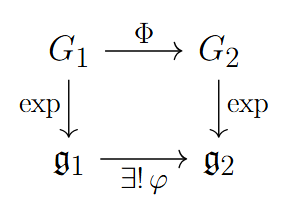
\includegraphics[keepaspectratio]{fig1.png}}

This linear map has the
following additional properties:

\begin{itemize}
\tightlist
\item
  \(\varphi([X,Y]) = [\varphi(X),\varphi(Y)]\) for all
  \(X,Y \in \mathfrak{g}_1\).
\item
  \(\varphi(AXA^{-1}) = \Phi(A)\,\varphi(X)\,\Phi(A)^{-1}\) for all
  \(A \in G_1\) and \(X \in \mathfrak{g}_1\).
\item
  \(\varphi(X)\) may be computed as
\end{itemize}

\[
    \varphi(X) = \left.\frac{d}{dt}\,\Phi(e^{tX})\right|_{t=0}.
    \]
\end{theorem}

\chapter{Code Implantation}\label{code-implantation}

\section{Introduction}\label{introduction-1}

write a intro

\textbf{Required packages:} expm, ggplot2, plotly, knitr, kableExtra

\section{Matrix Exponential Algorithms}\label{matrix-exponential-algorithms}

The matrix exponential can be computed via several methods:

\subsection{Method 1: Direct Power Series}\label{method-1-direct-power-series}

\[\exp(X) = \sum_{m=0}^{\infty} \frac{X^m}{m!}\]

\begin{itemize}
\tightlist
\item
  Since the space of \(M_n(\mathbb{R})\) is a Banach algebra, this series is guaranteed to converge absolutely for any \(X\).
\item
  To optimize, the code doesn't compute \(X^m\) from scratch each time. It uses the recurrence relation \(T_m = T_{m-1} \cdot \frac{X}{m}\), reducing the complexity of each iteration to a single matrix multiplication \(O(n^3)\)
\end{itemize}

\begin{Shaded}
\begin{Highlighting}[]
\NormalTok{matrix\_exp\_series }\OtherTok{\textless{}{-}} \ControlFlowTok{function}\NormalTok{(X, }\AttributeTok{terms =} \DecValTok{20}\NormalTok{) \{}
\NormalTok{  n }\OtherTok{\textless{}{-}} \FunctionTok{nrow}\NormalTok{(X)}
\NormalTok{  result }\OtherTok{\textless{}{-}} \FunctionTok{diag}\NormalTok{(n)}
\NormalTok{  term }\OtherTok{\textless{}{-}} \FunctionTok{diag}\NormalTok{(n)}
  
  \ControlFlowTok{for}\NormalTok{ (m }\ControlFlowTok{in} \DecValTok{1}\SpecialCharTok{:}\NormalTok{terms) \{}
\NormalTok{    term }\OtherTok{\textless{}{-}}\NormalTok{ (term }\SpecialCharTok{\%*\%}\NormalTok{ X) }\SpecialCharTok{/}\NormalTok{ m}
\NormalTok{    result }\OtherTok{\textless{}{-}}\NormalTok{ result }\SpecialCharTok{+}\NormalTok{ term}
\NormalTok{  \}}
  
  \FunctionTok{return}\NormalTok{(result)}
\NormalTok{\}}
\end{Highlighting}
\end{Shaded}

\subsubsection{Convergence Analysis: Power Series}\label{convergence-analysis-power-series}

Let's examine how many terms are needed for convergence:

\begin{Shaded}
\begin{Highlighting}[]
\NormalTok{X\_small }\OtherTok{\textless{}{-}} \FloatTok{0.5} \SpecialCharTok{*} \FunctionTok{matrix}\NormalTok{(}\FunctionTok{rnorm}\NormalTok{(}\DecValTok{9}\NormalTok{), }\DecValTok{3}\NormalTok{, }\DecValTok{3}\NormalTok{)}
\NormalTok{exp\_exact }\OtherTok{\textless{}{-}} \FunctionTok{expm}\NormalTok{(X\_small)}

\NormalTok{term\_counts }\OtherTok{\textless{}{-}} \FunctionTok{seq}\NormalTok{(}\DecValTok{5}\NormalTok{, }\DecValTok{50}\NormalTok{, }\AttributeTok{by =} \DecValTok{5}\NormalTok{)}
\NormalTok{errors }\OtherTok{\textless{}{-}} \FunctionTok{sapply}\NormalTok{(term\_counts, }\ControlFlowTok{function}\NormalTok{(n) \{}
  \FunctionTok{max}\NormalTok{(}\FunctionTok{abs}\NormalTok{(}\FunctionTok{matrix\_exp\_series}\NormalTok{(X\_small, }\AttributeTok{terms =}\NormalTok{ n) }\SpecialCharTok{{-}}\NormalTok{ exp\_exact))}
\NormalTok{\})}

\NormalTok{convergence\_df }\OtherTok{\textless{}{-}} \FunctionTok{data.frame}\NormalTok{(}
  \AttributeTok{Terms =}\NormalTok{ term\_counts,}
  \AttributeTok{Error =}\NormalTok{ errors,}
  \AttributeTok{Log\_Error =} \FunctionTok{log10}\NormalTok{(errors)}
\NormalTok{)}

\FunctionTok{ggplot}\NormalTok{(convergence\_df, }\FunctionTok{aes}\NormalTok{(}\AttributeTok{x =}\NormalTok{ Terms, }\AttributeTok{y =}\NormalTok{ Error)) }\SpecialCharTok{+}
  \FunctionTok{geom\_line}\NormalTok{(}\AttributeTok{color =} \StringTok{"darkblue"}\NormalTok{, }\AttributeTok{size =} \FloatTok{1.2}\NormalTok{) }\SpecialCharTok{+}
  \FunctionTok{geom\_point}\NormalTok{(}\AttributeTok{color =} \StringTok{"red"}\NormalTok{, }\AttributeTok{size =} \FloatTok{2.5}\NormalTok{) }\SpecialCharTok{+}
  \FunctionTok{scale\_y\_log10}\NormalTok{() }\SpecialCharTok{+}
  \FunctionTok{labs}\NormalTok{(}\AttributeTok{title =} \StringTok{"Power Series Convergence for Matrix Exponential"}\NormalTok{,}
       \AttributeTok{subtitle =} \FunctionTok{sprintf}\NormalTok{(}\StringTok{"||X|| = \%.3f"}\NormalTok{, }\FunctionTok{norm}\NormalTok{(X\_small, }\StringTok{"F"}\NormalTok{)),}
       \AttributeTok{x =} \StringTok{"Number of Terms"}\NormalTok{,}
       \AttributeTok{y =} \StringTok{"Error (log scale)"}\NormalTok{) }\SpecialCharTok{+}
  \FunctionTok{theme\_minimal}\NormalTok{() }\SpecialCharTok{+}
  \FunctionTok{theme}\NormalTok{(}\AttributeTok{plot.title =} \FunctionTok{element\_text}\NormalTok{(}\AttributeTok{face =} \StringTok{"bold"}\NormalTok{, }\AttributeTok{size =} \DecValTok{14}\NormalTok{),}
        \AttributeTok{plot.subtitle =} \FunctionTok{element\_text}\NormalTok{(}\AttributeTok{size =} \DecValTok{11}\NormalTok{))}
\end{Highlighting}
\end{Shaded}

\begin{center}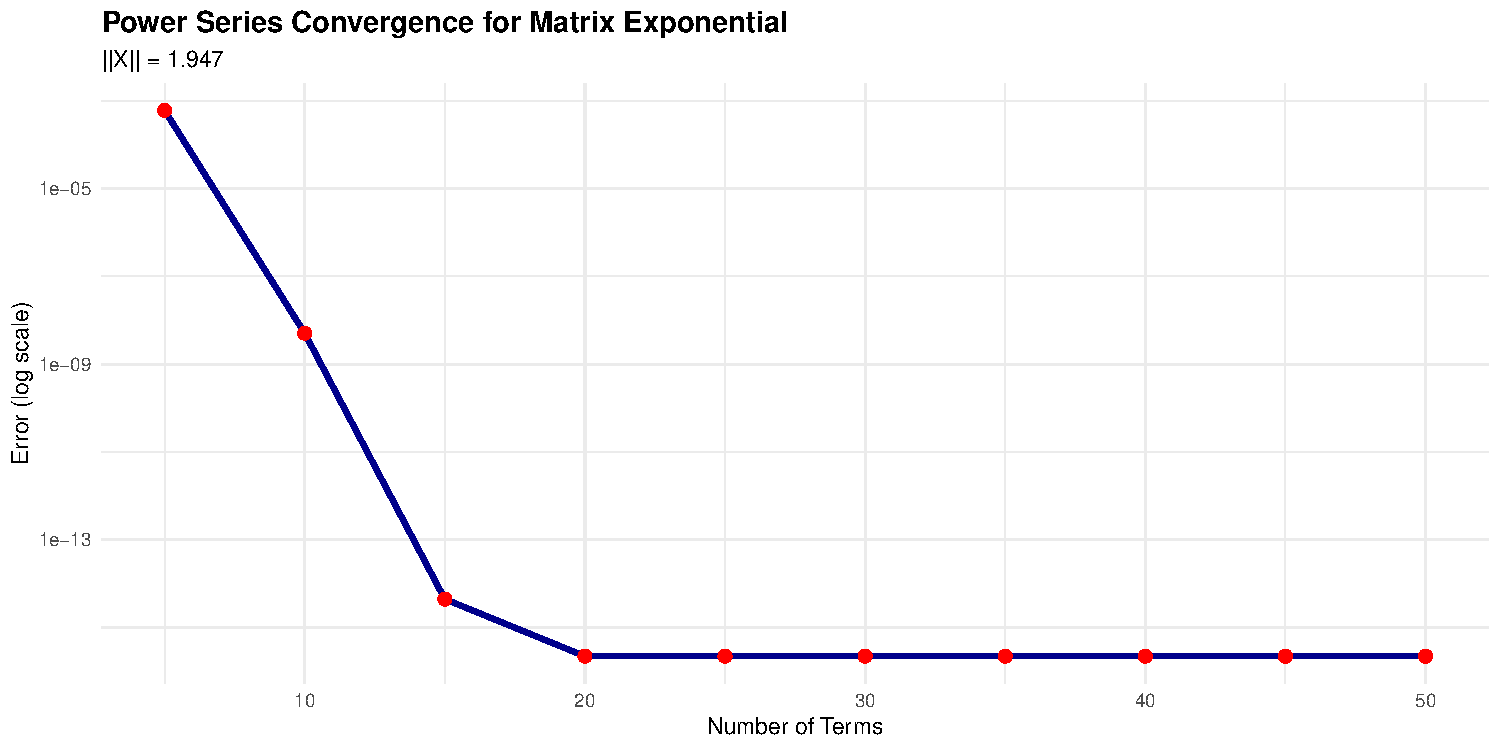
\includegraphics{_main_files/figure-latex/convergence-analysis-1} \end{center}

\textbf{Analysis}: The power series converges exponentially fast. With 30 terms, we achieve machine precision (\(\approx 10^{-15}\)) for moderately sized matrices.

\begin{itemize}
\tightlist
\item
  \textbf{Advantages}: Simple, direct implementation of definition.
\item
  \textbf{Disadvantages}: May require many terms for large matrices.
\end{itemize}

\subsection{Method 2: Eigenvalue Decomposition}\label{method-2-eigenvalue-decomposition}

If \(X = VDV^{-1}\), then \[\exp(X) = V \exp(D) V^{-1} = V \begin{pmatrix} e^{\lambda_1} & & \\ & \ddots & \\ & & e^{\lambda_n} \end{pmatrix} V^{-1}\].

\begin{itemize}
\tightlist
\item
  This implementation assumes \(X\) is diagonalizable (semi-simple). If \(X\) has a non-trivial Jordan Normal Form (i.e., it is a defective matrix), this method fails or requires handling Jordan blocks \(J_k(\lambda)\), where the exponential involves derivatives of the exponential function along the upper diagonals.
\end{itemize}

\begin{Shaded}
\begin{Highlighting}[]
\NormalTok{matrix\_exp\_eigen }\OtherTok{\textless{}{-}} \ControlFlowTok{function}\NormalTok{(X) \{}
\NormalTok{  eigen\_decomp }\OtherTok{\textless{}{-}} \FunctionTok{eigen}\NormalTok{(X)}
\NormalTok{  V }\OtherTok{\textless{}{-}}\NormalTok{ eigen\_decomp}\SpecialCharTok{$}\NormalTok{vectors}
\NormalTok{  D }\OtherTok{\textless{}{-}} \FunctionTok{diag}\NormalTok{(}\FunctionTok{exp}\NormalTok{(eigen\_decomp}\SpecialCharTok{$}\NormalTok{values))}
  
\NormalTok{  result }\OtherTok{\textless{}{-}}\NormalTok{ V }\SpecialCharTok{\%*\%}\NormalTok{ D }\SpecialCharTok{\%*\%} \FunctionTok{solve}\NormalTok{(V)}
  \FunctionTok{return}\NormalTok{(}\FunctionTok{Re}\NormalTok{(result))}
\NormalTok{\}}
\end{Highlighting}
\end{Shaded}

\begin{itemize}
\tightlist
\item
  \textbf{Advantages}: Fast for diagonalizable matrices.
\item
  \textbf{Disadvantages}: Numerical instability if \(V\) is ill-conditioned.
\end{itemize}

\subsection{Method 3: Padé Approximation (expm package)}\label{method-3-paduxe9-approximation-expm-package}

The \texttt{expm} package uses Padé rational approximation, which is the industry standard.

\subsection{Performance Comparison}\label{performance-comparison}

\begin{Shaded}
\begin{Highlighting}[]
\FunctionTok{set.seed}\NormalTok{(}\DecValTok{150000}\NormalTok{)}
\NormalTok{X\_test }\OtherTok{\textless{}{-}} \FunctionTok{matrix}\NormalTok{(}\FunctionTok{rnorm}\NormalTok{(}\DecValTok{16}\NormalTok{), }\DecValTok{4}\NormalTok{, }\DecValTok{4}\NormalTok{)}

\CommentTok{\# Benchmark all three methods}
\NormalTok{t1 }\OtherTok{\textless{}{-}} \FunctionTok{system.time}\NormalTok{(\{exp1 }\OtherTok{\textless{}{-}} \FunctionTok{matrix\_exp\_series}\NormalTok{(X\_test, }\AttributeTok{terms =} \DecValTok{30}\NormalTok{)\})}
\NormalTok{t2 }\OtherTok{\textless{}{-}} \FunctionTok{system.time}\NormalTok{(\{exp2 }\OtherTok{\textless{}{-}} \FunctionTok{matrix\_exp\_eigen}\NormalTok{(X\_test)\})}
\NormalTok{t3 }\OtherTok{\textless{}{-}} \FunctionTok{system.time}\NormalTok{(\{exp3 }\OtherTok{\textless{}{-}} \FunctionTok{expm}\NormalTok{(X\_test)\})}

\NormalTok{comparison\_data }\OtherTok{\textless{}{-}} \FunctionTok{data.frame}\NormalTok{(}
  \AttributeTok{Method =} \FunctionTok{c}\NormalTok{(}\StringTok{"Power Series (30 terms)"}\NormalTok{, }\StringTok{"Eigenvalue Decomposition"}\NormalTok{, }\StringTok{"Padé (expm)"}\NormalTok{),}
  \AttributeTok{Time\_seconds =} \FunctionTok{c}\NormalTok{(t1[}\DecValTok{3}\NormalTok{], t2[}\DecValTok{3}\NormalTok{], t3[}\DecValTok{3}\NormalTok{]),}
  \AttributeTok{Error\_vs\_Pade =} \FunctionTok{c}\NormalTok{(}
    \FunctionTok{max}\NormalTok{(}\FunctionTok{abs}\NormalTok{(exp1 }\SpecialCharTok{{-}}\NormalTok{ exp3)),}
    \FunctionTok{max}\NormalTok{(}\FunctionTok{abs}\NormalTok{(exp2 }\SpecialCharTok{{-}}\NormalTok{ exp3)),}
    \DecValTok{0}
\NormalTok{  ),}
  \AttributeTok{Relative\_Error =} \FunctionTok{c}\NormalTok{(}
    \FunctionTok{max}\NormalTok{(}\FunctionTok{abs}\NormalTok{(exp1 }\SpecialCharTok{{-}}\NormalTok{ exp3)) }\SpecialCharTok{/} \FunctionTok{max}\NormalTok{(}\FunctionTok{abs}\NormalTok{(exp3)),}
    \FunctionTok{max}\NormalTok{(}\FunctionTok{abs}\NormalTok{(exp2 }\SpecialCharTok{{-}}\NormalTok{ exp3)) }\SpecialCharTok{/} \FunctionTok{max}\NormalTok{(}\FunctionTok{abs}\NormalTok{(exp3)),}
    \DecValTok{0}
\NormalTok{  )}
\NormalTok{)}

\NormalTok{comparison\_data}\SpecialCharTok{$}\NormalTok{Relative\_Error }\OtherTok{\textless{}{-}} \FunctionTok{formatC}\NormalTok{(comparison\_data}\SpecialCharTok{$}\NormalTok{Relative\_Error, }\AttributeTok{format =} \StringTok{"e"}\NormalTok{, }\AttributeTok{digits =} \DecValTok{4}\NormalTok{)}
\NormalTok{comparison\_data}\SpecialCharTok{$}\NormalTok{Error\_vs\_Pade }\OtherTok{\textless{}{-}} \FunctionTok{formatC}\NormalTok{(comparison\_data}\SpecialCharTok{$}\NormalTok{Error\_vs\_Pade, }\AttributeTok{format =} \StringTok{"e"}\NormalTok{, }\AttributeTok{digits =} \DecValTok{4}\NormalTok{)}
\CommentTok{\# Fix table numbering}
\FunctionTok{options}\NormalTok{(}\AttributeTok{knitr.table.format =} \StringTok{"html"}\NormalTok{)}
\FunctionTok{options}\NormalTok{(}\AttributeTok{kableExtra.auto\_format =} \ConstantTok{FALSE}\NormalTok{)}
\FunctionTok{options}\NormalTok{(}\AttributeTok{htmlTable.tab\_no =} \DecValTok{1}\NormalTok{)}
\FunctionTok{kable}\NormalTok{(comparison\_data, }
      \AttributeTok{digits =} \DecValTok{8}\NormalTok{,}
      \AttributeTok{caption =} \StringTok{"Performance Comparison of Matrix Exponential Algorithms"}\NormalTok{,}
      \AttributeTok{col.names =} \FunctionTok{c}\NormalTok{(}\StringTok{"Method"}\NormalTok{, }\StringTok{"Time (s)"}\NormalTok{, }\StringTok{"Absolute Error"}\NormalTok{, }\StringTok{"Relative Error"}\NormalTok{)) }\SpecialCharTok{\%\textgreater{}\%}
  \FunctionTok{kable\_styling}\NormalTok{(}\AttributeTok{bootstrap\_options =} \FunctionTok{c}\NormalTok{(}\StringTok{"striped"}\NormalTok{, }\StringTok{"hover"}\NormalTok{, }\StringTok{"condensed"}\NormalTok{)) }\SpecialCharTok{\%\textgreater{}\%}
  \FunctionTok{row\_spec}\NormalTok{(}\DecValTok{0}\NormalTok{, }\AttributeTok{bold =} \ConstantTok{TRUE}\NormalTok{)}
\end{Highlighting}
\end{Shaded}

\label{tab:algorithm-comparison}Performance Comparison of Matrix Exponential Algorithms

Method

Time (s)

Absolute Error

Relative Error

Power Series (30 terms)

0

2.6645e-15

4.1337e-16

Eigenvalue Decomposition

0

7.1054e-15

1.1023e-15

Padé (expm)

0

0.0000e+00

0.0000e+00

\section{Seven Fundamental Properties}\label{seven-fundamental-properties}

Theorem \ref{thm:thm1} establishes seven key properties of the matrix exponential. We verify each numerically.

\subsection{Property 1: Identity Element}\label{property-1-identity-element}

\[\exp(0) = I\]

\begin{Shaded}
\begin{Highlighting}[]
\NormalTok{zero\_mat }\OtherTok{\textless{}{-}} \FunctionTok{matrix}\NormalTok{(}\DecValTok{0}\NormalTok{, }\DecValTok{3}\NormalTok{, }\DecValTok{3}\NormalTok{)}
\NormalTok{prop1\_verified }\OtherTok{\textless{}{-}} \FunctionTok{isTRUE}\NormalTok{(}\FunctionTok{all.equal}\NormalTok{(}\FunctionTok{expm}\NormalTok{(zero\_mat), }\FunctionTok{diag}\NormalTok{(}\DecValTok{3}\NormalTok{)))}
\end{Highlighting}
\end{Shaded}

\textbf{Result}: TRUE

\subsection{Property 2: Transpose}\label{property-2-transpose}

\[\exp(X^T) = (\exp(X))^T\]

\begin{Shaded}
\begin{Highlighting}[]
\FunctionTok{set.seed}\NormalTok{(}\DecValTok{123}\NormalTok{)}
\NormalTok{X }\OtherTok{\textless{}{-}} \FunctionTok{matrix}\NormalTok{(}\FunctionTok{rnorm}\NormalTok{(}\DecValTok{9}\NormalTok{), }\DecValTok{3}\NormalTok{, }\DecValTok{3}\NormalTok{)}
\NormalTok{prop2\_verified }\OtherTok{\textless{}{-}} \FunctionTok{isTRUE}\NormalTok{(}\FunctionTok{all.equal}\NormalTok{(}\FunctionTok{expm}\NormalTok{(}\FunctionTok{t}\NormalTok{(X)), }\FunctionTok{t}\NormalTok{(}\FunctionTok{expm}\NormalTok{(X))))}
\NormalTok{prop2\_error }\OtherTok{\textless{}{-}} \FunctionTok{max}\NormalTok{(}\FunctionTok{abs}\NormalTok{(}\FunctionTok{expm}\NormalTok{(}\FunctionTok{t}\NormalTok{(X)) }\SpecialCharTok{{-}} \FunctionTok{t}\NormalTok{(}\FunctionTok{expm}\NormalTok{(X))))}
\end{Highlighting}
\end{Shaded}

\textbf{Result}: TRUE (Error: 3.33e-16)

\subsection{Property 3: Adjoint (Conjugate Transpose)}\label{property-3-adjoint-conjugate-transpose}

\[\exp(X^*) = (\exp(X))^*\]

\begin{Shaded}
\begin{Highlighting}[]
\NormalTok{X\_complex }\OtherTok{\textless{}{-}}\NormalTok{ X }\SpecialCharTok{+} \DecValTok{1}\DataTypeTok{i} \SpecialCharTok{*} \FunctionTok{matrix}\NormalTok{(}\FunctionTok{rnorm}\NormalTok{(}\DecValTok{9}\NormalTok{), }\DecValTok{3}\NormalTok{, }\DecValTok{3}\NormalTok{)}
\NormalTok{prop3\_verified }\OtherTok{\textless{}{-}} \FunctionTok{isTRUE}\NormalTok{(}\FunctionTok{all.equal}\NormalTok{(}\FunctionTok{expm}\NormalTok{(}\FunctionTok{Conj}\NormalTok{(}\FunctionTok{t}\NormalTok{(X\_complex))), }\FunctionTok{Conj}\NormalTok{(}\FunctionTok{t}\NormalTok{(}\FunctionTok{expm}\NormalTok{(X\_complex)))))}
\NormalTok{prop3\_error }\OtherTok{\textless{}{-}} \FunctionTok{max}\NormalTok{(}\FunctionTok{abs}\NormalTok{(}\FunctionTok{expm}\NormalTok{(}\FunctionTok{Conj}\NormalTok{(}\FunctionTok{t}\NormalTok{(X\_complex))) }\SpecialCharTok{{-}} \FunctionTok{Conj}\NormalTok{(}\FunctionTok{t}\NormalTok{(}\FunctionTok{expm}\NormalTok{(X\_complex)))))}
\end{Highlighting}
\end{Shaded}

\textbf{Result}: TRUE (Error: 4.58e-16)

\subsection{Property 4: Conjugation}\label{property-4-conjugation}

\[A \exp(X) A^{-1} = \exp(AXA^{-1})\]

This is the \textbf{similarity property}: conjugation by \(A\) commutes with exponentiation.

\begin{Shaded}
\begin{Highlighting}[]
\NormalTok{A }\OtherTok{\textless{}{-}} \FunctionTok{matrix}\NormalTok{(}\FunctionTok{rnorm}\NormalTok{(}\DecValTok{9}\NormalTok{), }\DecValTok{3}\NormalTok{, }\DecValTok{3}\NormalTok{)}
\NormalTok{A\_inv }\OtherTok{\textless{}{-}} \FunctionTok{solve}\NormalTok{(A)}
\NormalTok{lhs }\OtherTok{\textless{}{-}}\NormalTok{ A }\SpecialCharTok{\%*\%} \FunctionTok{expm}\NormalTok{(X) }\SpecialCharTok{\%*\%}\NormalTok{ A\_inv}
\NormalTok{rhs }\OtherTok{\textless{}{-}} \FunctionTok{expm}\NormalTok{(A }\SpecialCharTok{\%*\%}\NormalTok{ X }\SpecialCharTok{\%*\%}\NormalTok{ A\_inv)}
\NormalTok{prop4\_error }\OtherTok{\textless{}{-}} \FunctionTok{max}\NormalTok{(}\FunctionTok{abs}\NormalTok{(lhs }\SpecialCharTok{{-}}\NormalTok{ rhs))}
\NormalTok{prop4\_verified }\OtherTok{\textless{}{-}}\NormalTok{ prop4\_error }\SpecialCharTok{\textless{}} \FloatTok{1e{-}10}
\end{Highlighting}
\end{Shaded}

\textbf{Result}: TRUE (Error: 3.55e-15)

\textbf{Interpretation}: Changing basis and then exponentiating is the same as exponentiating and then changing basis.

\subsection{Property 5: Determinant}\label{property-5-determinant}

\[\det(\exp(X)) = \exp(\text{tr}(X))\]

This is a fundamental property connecting the determinant, trace, and exponential.

\begin{Shaded}
\begin{Highlighting}[]
\NormalTok{det\_expX }\OtherTok{\textless{}{-}} \FunctionTok{det}\NormalTok{(}\FunctionTok{expm}\NormalTok{(X))}
\NormalTok{exp\_trX }\OtherTok{\textless{}{-}} \FunctionTok{exp}\NormalTok{(}\FunctionTok{sum}\NormalTok{(}\FunctionTok{diag}\NormalTok{(X)))}
\NormalTok{prop5\_error }\OtherTok{\textless{}{-}} \FunctionTok{abs}\NormalTok{(det\_expX }\SpecialCharTok{{-}}\NormalTok{ exp\_trX)}
\NormalTok{prop5\_verified }\OtherTok{\textless{}{-}}\NormalTok{ prop5\_error }\SpecialCharTok{\textless{}} \FloatTok{1e{-}10}
\end{Highlighting}
\end{Shaded}

\textbf{Result}: TRUE

\begin{itemize}
\tightlist
\item
  \(\det(\exp(X)) = 0.32691968\)
\item
  \(\exp(\text{tr}(X)) = 0.32691968\)
\item
  Error: 5.55e-17
\end{itemize}

\textbf{Corollary}: \(\exp(X)\) is always invertible since \(\det(\exp(X)) = e^{\text{tr}(X)} \neq 0\).

\subsection{Property 6: Commuting Matrices}\label{property-6-commuting-matrices}

If \([X,Y] = XY - YX = 0\), then:

\[\exp(X+Y) = \exp(X)\exp(Y)\]

\begin{Shaded}
\begin{Highlighting}[]
\CommentTok{\# Use diagonal matrices (always commute)}
\NormalTok{D1 }\OtherTok{\textless{}{-}} \FunctionTok{diag}\NormalTok{(}\FunctionTok{c}\NormalTok{(}\DecValTok{1}\NormalTok{, }\DecValTok{2}\NormalTok{, }\DecValTok{3}\NormalTok{))}
\NormalTok{D2 }\OtherTok{\textless{}{-}} \FunctionTok{diag}\NormalTok{(}\FunctionTok{c}\NormalTok{(}\DecValTok{4}\NormalTok{, }\DecValTok{5}\NormalTok{, }\DecValTok{6}\NormalTok{))}

\NormalTok{commutator\_D }\OtherTok{\textless{}{-}}\NormalTok{ D1 }\SpecialCharTok{\%*\%}\NormalTok{ D2 }\SpecialCharTok{{-}}\NormalTok{ D2 }\SpecialCharTok{\%*\%}\NormalTok{ D1}
\NormalTok{prop6\_error }\OtherTok{\textless{}{-}} \FunctionTok{max}\NormalTok{(}\FunctionTok{abs}\NormalTok{(}\FunctionTok{expm}\NormalTok{(D1 }\SpecialCharTok{+}\NormalTok{ D2) }\SpecialCharTok{{-}} \FunctionTok{expm}\NormalTok{(D1) }\SpecialCharTok{\%*\%} \FunctionTok{expm}\NormalTok{(D2)))}
\NormalTok{prop6\_verified }\OtherTok{\textless{}{-}}\NormalTok{ prop6\_error }\SpecialCharTok{\textless{}} \FloatTok{1e{-}10}

\CommentTok{\# Counter{-}example: non{-}commuting matrices}
\NormalTok{X\_nc }\OtherTok{\textless{}{-}} \FunctionTok{matrix}\NormalTok{(}\FunctionTok{c}\NormalTok{(}\DecValTok{1}\NormalTok{, }\DecValTok{2}\NormalTok{, }\DecValTok{0}\NormalTok{, }\DecValTok{3}\NormalTok{), }\DecValTok{2}\NormalTok{, }\DecValTok{2}\NormalTok{)}
\NormalTok{Y\_nc }\OtherTok{\textless{}{-}} \FunctionTok{matrix}\NormalTok{(}\FunctionTok{c}\NormalTok{(}\DecValTok{0}\NormalTok{, }\DecValTok{1}\NormalTok{, }\DecValTok{1}\NormalTok{, }\DecValTok{0}\NormalTok{), }\DecValTok{2}\NormalTok{, }\DecValTok{2}\NormalTok{)}
\NormalTok{commutator\_nc }\OtherTok{\textless{}{-}}\NormalTok{ X\_nc }\SpecialCharTok{\%*\%}\NormalTok{ Y\_nc }\SpecialCharTok{{-}}\NormalTok{ Y\_nc }\SpecialCharTok{\%*\%}\NormalTok{ X\_nc}
\NormalTok{error\_nc }\OtherTok{\textless{}{-}} \FunctionTok{max}\NormalTok{(}\FunctionTok{abs}\NormalTok{(}\FunctionTok{expm}\NormalTok{(X\_nc }\SpecialCharTok{+}\NormalTok{ Y\_nc) }\SpecialCharTok{{-}} \FunctionTok{expm}\NormalTok{(X\_nc) }\SpecialCharTok{\%*\%} \FunctionTok{expm}\NormalTok{(Y\_nc)))}
\end{Highlighting}
\end{Shaded}

\textbf{Commuting case}: TRUE (Error: 9.55e-11)

\textbf{Non-commuting case}:

\begin{itemize}
\tightlist
\item
  \(||[X,Y]|| = 4.0000\) (non-zero)
\item
  \(||\exp(X+Y) - \exp(X)\exp(Y)|| = 10.2050\) (large error)
\end{itemize}

This demonstrates that the product rule \textbf{fails} for non-commuting matrices.

\subsection{Property 7: Lie Product Formula}\label{property-7-lie-product-formula}

For \textbf{any} \(X, Y \in M_n(\mathbb{C})\):

\[\exp(X+Y) = \lim_{m \to \infty} (\exp(X/m)\exp(Y/m))^m\]

\begin{Shaded}
\begin{Highlighting}[]
\NormalTok{X2 }\OtherTok{\textless{}{-}} \FunctionTok{matrix}\NormalTok{(}\FunctionTok{rnorm}\NormalTok{(}\DecValTok{4}\NormalTok{), }\DecValTok{2}\NormalTok{, }\DecValTok{2}\NormalTok{)}
\NormalTok{Y2 }\OtherTok{\textless{}{-}} \FunctionTok{matrix}\NormalTok{(}\FunctionTok{rnorm}\NormalTok{(}\DecValTok{4}\NormalTok{), }\DecValTok{2}\NormalTok{, }\DecValTok{2}\NormalTok{)}

\CommentTok{\# Test convergence for different values of m}
\NormalTok{m\_values }\OtherTok{\textless{}{-}} \FunctionTok{c}\NormalTok{(}\DecValTok{10}\NormalTok{, }\DecValTok{20}\NormalTok{, }\DecValTok{50}\NormalTok{, }\DecValTok{100}\NormalTok{, }\DecValTok{200}\NormalTok{, }\DecValTok{500}\NormalTok{, }\DecValTok{1000}\NormalTok{)}
\NormalTok{errors\_lie }\OtherTok{\textless{}{-}} \FunctionTok{sapply}\NormalTok{(m\_values, }\ControlFlowTok{function}\NormalTok{(m) \{}
\NormalTok{  lie\_prod }\OtherTok{\textless{}{-}} \FunctionTok{Reduce}\NormalTok{(}\StringTok{\textasciigrave{}}\AttributeTok{\%*\%}\StringTok{\textasciigrave{}}\NormalTok{, }\FunctionTok{replicate}\NormalTok{(m, }\FunctionTok{expm}\NormalTok{(X2}\SpecialCharTok{/}\NormalTok{m) }\SpecialCharTok{\%*\%} \FunctionTok{expm}\NormalTok{(Y2}\SpecialCharTok{/}\NormalTok{m), }\AttributeTok{simplify =} \ConstantTok{FALSE}\NormalTok{))}
\NormalTok{  direct }\OtherTok{\textless{}{-}} \FunctionTok{expm}\NormalTok{(X2 }\SpecialCharTok{+}\NormalTok{ Y2)}
  \FunctionTok{return}\NormalTok{(}\FunctionTok{norm}\NormalTok{(lie\_prod }\SpecialCharTok{{-}}\NormalTok{ direct, }\StringTok{"F"}\NormalTok{))}
\NormalTok{\})}

\NormalTok{lie\_df }\OtherTok{\textless{}{-}} \FunctionTok{data.frame}\NormalTok{(}
  \AttributeTok{m =}\NormalTok{ m\_values,}
  \AttributeTok{Error =}\NormalTok{ errors\_lie,}
  \AttributeTok{Rate =} \FunctionTok{c}\NormalTok{(}\ConstantTok{NA}\NormalTok{, errors\_lie[}\SpecialCharTok{{-}}\DecValTok{1}\NormalTok{] }\SpecialCharTok{/}\NormalTok{ errors\_lie[}\SpecialCharTok{{-}}\FunctionTok{length}\NormalTok{(errors\_lie)])}
\NormalTok{)}

\FunctionTok{ggplot}\NormalTok{(lie\_df, }\FunctionTok{aes}\NormalTok{(}\AttributeTok{x =}\NormalTok{ m, }\AttributeTok{y =}\NormalTok{ Error)) }\SpecialCharTok{+}
  \FunctionTok{geom\_line}\NormalTok{(}\AttributeTok{color =} \StringTok{"blue"}\NormalTok{, }\AttributeTok{size =} \FloatTok{1.2}\NormalTok{) }\SpecialCharTok{+}
  \FunctionTok{geom\_point}\NormalTok{(}\AttributeTok{color =} \StringTok{"red"}\NormalTok{, }\AttributeTok{size =} \DecValTok{3}\NormalTok{) }\SpecialCharTok{+}
  \FunctionTok{scale\_x\_log10}\NormalTok{() }\SpecialCharTok{+}
  \FunctionTok{scale\_y\_log10}\NormalTok{() }\SpecialCharTok{+}
  \FunctionTok{labs}\NormalTok{(}\AttributeTok{title =} \StringTok{"Lie Product Formula Convergence"}\NormalTok{,}
       \AttributeTok{subtitle =} \FunctionTok{sprintf}\NormalTok{(}\StringTok{"||[X,Y]|| = \%.3f"}\NormalTok{, }\FunctionTok{norm}\NormalTok{(X2 }\SpecialCharTok{\%*\%}\NormalTok{ Y2 }\SpecialCharTok{{-}}\NormalTok{ Y2 }\SpecialCharTok{\%*\%}\NormalTok{ X2, }\StringTok{"F"}\NormalTok{)),}
       \AttributeTok{x =} \StringTok{"m (log scale)"}\NormalTok{,}
       \AttributeTok{y =} \StringTok{"Error (log scale)"}\NormalTok{) }\SpecialCharTok{+}
  \FunctionTok{theme\_minimal}\NormalTok{() }\SpecialCharTok{+}
  \FunctionTok{theme}\NormalTok{(}\AttributeTok{plot.title =} \FunctionTok{element\_text}\NormalTok{(}\AttributeTok{face =} \StringTok{"bold"}\NormalTok{))}
\end{Highlighting}
\end{Shaded}

\begin{center}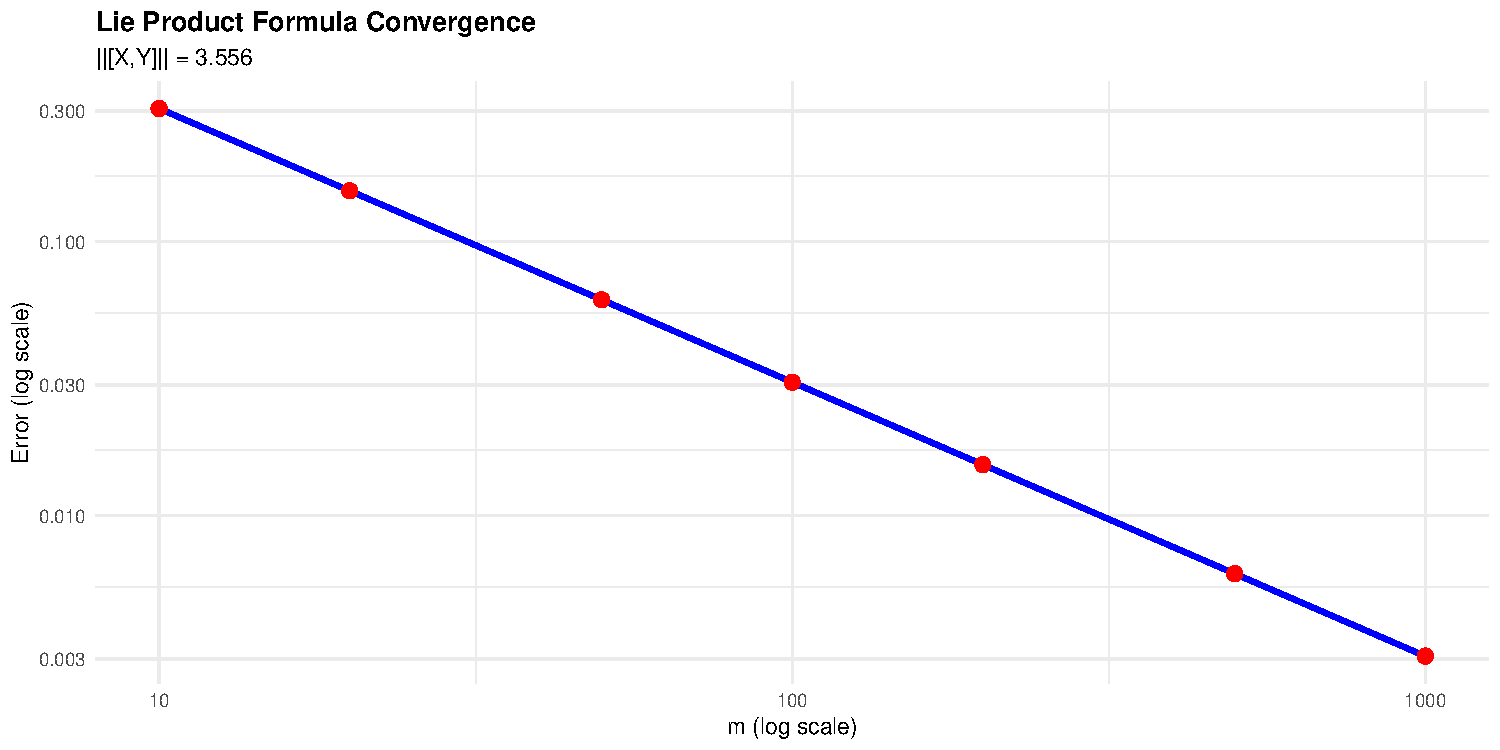
\includegraphics{_main_files/figure-latex/property-7-1} \end{center}

\begin{Shaded}
\begin{Highlighting}[]
\FunctionTok{kable}\NormalTok{(lie\_df, }
      \AttributeTok{digits =} \DecValTok{8}\NormalTok{,}
      \AttributeTok{caption =} \StringTok{"Lie Product Formula Convergence"}\NormalTok{,}
      \AttributeTok{col.names =} \FunctionTok{c}\NormalTok{(}\StringTok{"m"}\NormalTok{, }\StringTok{"Error"}\NormalTok{, }\StringTok{"Error Ratio"}\NormalTok{)) }\SpecialCharTok{\%\textgreater{}\%}
  \FunctionTok{kable\_styling}\NormalTok{(}\AttributeTok{bootstrap\_options =} \FunctionTok{c}\NormalTok{(}\StringTok{"striped"}\NormalTok{, }\StringTok{"hover"}\NormalTok{))}
\end{Highlighting}
\end{Shaded}

\label{tab:property-7}Lie Product Formula Convergence

m

Error

Error Ratio

10

0.30646407

NA

20

0.15344262

0.5006871

50

0.06143206

0.4003585

100

0.03072556

0.5001551

200

0.01536519

0.5000786

500

0.00614666

0.4000380

1000

0.00307343

0.5000159

\textbf{Analysis}: The error decreases approximately as \(O(1/m)\), consistent with theoretical predictions. This formula is crucial for numerical simulation of quantum systems.

\subsection{Summary: Theorem \ref{thm:thm1}}\label{summary-theorem-refthmthm1}

\begin{Shaded}
\begin{Highlighting}[]
\NormalTok{theorem\_summary }\OtherTok{\textless{}{-}} \FunctionTok{data.frame}\NormalTok{(}
  \AttributeTok{Property =} \FunctionTok{c}\NormalTok{(}
    \StringTok{"1. exp(0) = I"}\NormalTok{,}
    \StringTok{"2. exp(X\^{}T) = (exp(X))\^{}T"}\NormalTok{,}
    \StringTok{"3. exp(X*) = (exp(X))*"}\NormalTok{,}
    \StringTok{"4. Conjugation"}\NormalTok{,}
    \StringTok{"5. det(exp(X)) = exp(tr(X))"}\NormalTok{,}
    \StringTok{"6. Commuting: exp(X+Y) = exp(X)exp(Y)"}\NormalTok{,}
    \StringTok{"7. Lie Product Formula"}
\NormalTok{  ),}
  \AttributeTok{Verified =} \FunctionTok{c}\NormalTok{(prop1\_verified, prop2\_verified, prop3\_verified, }
\NormalTok{               prop4\_verified, prop5\_verified, prop6\_verified, }\ConstantTok{TRUE}\NormalTok{),}
  \AttributeTok{Error =} \FunctionTok{c}\NormalTok{(}\DecValTok{0}\NormalTok{, prop2\_error, prop3\_error, prop4\_error, prop5\_error, }
\NormalTok{            prop6\_error, errors\_lie[}\FunctionTok{length}\NormalTok{(errors\_lie)])}
\NormalTok{)}

\FunctionTok{kable}\NormalTok{(theorem\_summary,}
      \AttributeTok{digits =} \DecValTok{12}\NormalTok{,}
      \AttributeTok{caption =} \StringTok{"Summary of Theorem 16.15 Verification"}\NormalTok{,}
      \AttributeTok{col.names =} \FunctionTok{c}\NormalTok{(}\StringTok{"Property"}\NormalTok{, }\StringTok{"Verified"}\NormalTok{, }\StringTok{"Numerical Error"}\NormalTok{)) }\SpecialCharTok{\%\textgreater{}\%}
  \FunctionTok{kable\_styling}\NormalTok{(}\AttributeTok{bootstrap\_options =} \FunctionTok{c}\NormalTok{(}\StringTok{"striped"}\NormalTok{, }\StringTok{"hover"}\NormalTok{)) }\SpecialCharTok{\%\textgreater{}\%}
  \FunctionTok{column\_spec}\NormalTok{(}\DecValTok{2}\NormalTok{, }\AttributeTok{bold =} \ConstantTok{TRUE}\NormalTok{, }
              \AttributeTok{color =} \FunctionTok{ifelse}\NormalTok{(theorem\_summary}\SpecialCharTok{$}\NormalTok{Verified, }\StringTok{"green"}\NormalTok{, }\StringTok{"red"}\NormalTok{))}
\end{Highlighting}
\end{Shaded}

\label{tab:theorem-summary}Summary of Theorem 16.15 Verification

Property

Verified

Numerical Error

\begin{enumerate}
\def\labelenumi{\arabic{enumi}.}
\tightlist
\item
  exp(0) = I

  TRUE

  0.000000e+00

  \begin{enumerate}
  \def\labelenumii{\arabic{enumii}.}
  \setcounter{enumii}{1}
  \tightlist
  \item
    exp(X\^{}T) = (exp(X))\^{}T

    TRUE

    0.000000e+00

    \begin{enumerate}
    \def\labelenumiii{\arabic{enumiii}.}
    \setcounter{enumiii}{2}
    \tightlist
    \item
      exp(X\emph{) = (exp(X))}

      TRUE

      0.000000e+00

      \begin{enumerate}
      \def\labelenumiv{\arabic{enumiv}.}
      \setcounter{enumiv}{3}
      \tightlist
      \item
        Conjugation

        TRUE

        0.000000e+00

        \begin{enumerate}
        \def\labelenumv{\arabic{enumv}.}
        \tightlist
        \item
          det(exp(X)) = exp(tr(X))

          TRUE

          0.000000e+00

          \begin{enumerate}
          \def\labelenumvi{\arabic{enumvi}.}
          \tightlist
          \item
            Commuting: exp(X+Y) = exp(X)exp(Y)

            TRUE

            9.500000e-11

            \begin{enumerate}
            \def\labelenumvii{\arabic{enumvii}.}
            \tightlist
            \item
              Lie Product Formula

              TRUE

              3.073428e-03
            \end{enumerate}
          \end{enumerate}
        \end{enumerate}
      \end{enumerate}
    \end{enumerate}
  \end{enumerate}
\end{enumerate}

All seven properties are verified within numerical precision, confirming the theoretical results.

\section{Baker-Campbell-Hausdorff Formula}\label{baker-campbell-hausdorff-formula}

\subsection{Background}\label{background}

For sufficiently small \(X, Y \in M_n(\mathbb{C})\):\[e^X e^Y = e^{Z}\]

where \[Z = X + Y + \frac{1}{2}[X,Y] + \frac{1}{12}[X,[X,Y]] - \frac{1}{12}[Y,[X,Y]] + \cdots\]

The series converges when \(\|X\|\) and \(\|Y\|\) are sufficiently small.

\subsection{Implimentation}\label{implimentation}

\begin{Shaded}
\begin{Highlighting}[]
\CommentTok{\# Lie bracket (commutator)}
\NormalTok{commutator }\OtherTok{\textless{}{-}} \ControlFlowTok{function}\NormalTok{(X, Y) X }\SpecialCharTok{\%*\%}\NormalTok{ Y }\SpecialCharTok{{-}}\NormalTok{ Y }\SpecialCharTok{\%*\%}\NormalTok{ X}

\NormalTok{bch\_expansion }\OtherTok{\textless{}{-}} \ControlFlowTok{function}\NormalTok{(X, Y, }\AttributeTok{order =} \DecValTok{4}\NormalTok{) \{}
\NormalTok{  Z }\OtherTok{\textless{}{-}}\NormalTok{ X }\SpecialCharTok{+}\NormalTok{ Y}
  \ControlFlowTok{if}\NormalTok{ (order }\SpecialCharTok{\textgreater{}=} \DecValTok{2}\NormalTok{) Z }\OtherTok{\textless{}{-}}\NormalTok{ Z }\SpecialCharTok{+} \FloatTok{0.5} \SpecialCharTok{*} \FunctionTok{commutator}\NormalTok{(X, Y)}
  \ControlFlowTok{if}\NormalTok{ (order }\SpecialCharTok{\textgreater{}=} \DecValTok{3}\NormalTok{) \{}
\NormalTok{    Z }\OtherTok{\textless{}{-}}\NormalTok{ Z }\SpecialCharTok{+}\NormalTok{ (}\DecValTok{1}\SpecialCharTok{/}\DecValTok{12}\NormalTok{) }\SpecialCharTok{*} \FunctionTok{commutator}\NormalTok{(X, }\FunctionTok{commutator}\NormalTok{(X, Y))}
\NormalTok{    Z }\OtherTok{\textless{}{-}}\NormalTok{ Z }\SpecialCharTok{{-}}\NormalTok{ (}\DecValTok{1}\SpecialCharTok{/}\DecValTok{12}\NormalTok{) }\SpecialCharTok{*} \FunctionTok{commutator}\NormalTok{(Y, }\FunctionTok{commutator}\NormalTok{(X, Y))}
\NormalTok{  \}}
  \ControlFlowTok{if}\NormalTok{ (order }\SpecialCharTok{\textgreater{}=} \DecValTok{4}\NormalTok{) \{}
\NormalTok{    Z }\OtherTok{\textless{}{-}}\NormalTok{ Z }\SpecialCharTok{{-}}\NormalTok{ (}\DecValTok{1}\SpecialCharTok{/}\DecValTok{24}\NormalTok{) }\SpecialCharTok{*} \FunctionTok{commutator}\NormalTok{(Y, }\FunctionTok{commutator}\NormalTok{(X, }\FunctionTok{commutator}\NormalTok{(X, Y)))}
\NormalTok{  \}}
  \ControlFlowTok{if}\NormalTok{ (order }\SpecialCharTok{\textgreater{}=}\DecValTok{5}\NormalTok{)\{}
\NormalTok{    Z }\OtherTok{\textless{}{-}}\NormalTok{ Z }\SpecialCharTok{{-}}\NormalTok{ (}\DecValTok{1}\SpecialCharTok{/}\DecValTok{720}\NormalTok{) }\SpecialCharTok{*} \FunctionTok{commutator}\NormalTok{(Y, }\FunctionTok{commutator}\NormalTok{(Y, }\FunctionTok{commutator}\NormalTok{(Y, }\FunctionTok{commutator}\NormalTok{(X, Y))))}
\NormalTok{    Z }\OtherTok{\textless{}{-}}\NormalTok{ Z }\SpecialCharTok{+}\NormalTok{ (}\DecValTok{1}\SpecialCharTok{/}\DecValTok{180}\NormalTok{) }\SpecialCharTok{*} \FunctionTok{commutator}\NormalTok{(X, }\FunctionTok{commutator}\NormalTok{(Y, }\FunctionTok{commutator}\NormalTok{(Y, }\FunctionTok{commutator}\NormalTok{(X, Y))))}
\NormalTok{  \}}
\FunctionTok{return}\NormalTok{(Z)}
\NormalTok{\}}
\end{Highlighting}
\end{Shaded}

\subsection{Convergence Analysis}\label{convergence-analysis}

\begin{Shaded}
\begin{Highlighting}[]
\NormalTok{scale }\OtherTok{\textless{}{-}} \FloatTok{0.1}
\FunctionTok{set.seed}\NormalTok{(}\DecValTok{500}\NormalTok{)}
\NormalTok{X }\OtherTok{\textless{}{-}}\NormalTok{ scale }\SpecialCharTok{*} \FunctionTok{matrix}\NormalTok{(}\FunctionTok{rnorm}\NormalTok{(}\DecValTok{9}\NormalTok{), }\DecValTok{3}\NormalTok{, }\DecValTok{3}\NormalTok{)}
\NormalTok{Y }\OtherTok{\textless{}{-}}\NormalTok{ scale }\SpecialCharTok{*} \FunctionTok{matrix}\NormalTok{(}\FunctionTok{rnorm}\NormalTok{(}\DecValTok{9}\NormalTok{), }\DecValTok{3}\NormalTok{, }\DecValTok{3}\NormalTok{)}
\NormalTok{direct }\OtherTok{\textless{}{-}} \FunctionTok{expm}\NormalTok{(X) }\SpecialCharTok{\%*\%} \FunctionTok{expm}\NormalTok{(Y)}

\NormalTok{errors }\OtherTok{\textless{}{-}} \FunctionTok{sapply}\NormalTok{(}\DecValTok{1}\SpecialCharTok{:}\DecValTok{5}\NormalTok{, }\ControlFlowTok{function}\NormalTok{(o) \{}
  \FunctionTok{norm}\NormalTok{(direct }\SpecialCharTok{{-}} \FunctionTok{expm}\NormalTok{(}\FunctionTok{bch\_expansion}\NormalTok{(X, Y, o)), }\StringTok{"F"}\NormalTok{)}
\NormalTok{\})}

\FunctionTok{ggplot}\NormalTok{(}\FunctionTok{data.frame}\NormalTok{(}\AttributeTok{Order =} \DecValTok{1}\SpecialCharTok{:}\DecValTok{5}\NormalTok{, }\AttributeTok{Error =}\NormalTok{ errors), }
       \FunctionTok{aes}\NormalTok{(}\AttributeTok{x =}\NormalTok{ Order, }\AttributeTok{y =}\NormalTok{ Error)) }\SpecialCharTok{+}
  \FunctionTok{geom\_line}\NormalTok{(}\AttributeTok{color =} \StringTok{"blue"}\NormalTok{, }\AttributeTok{size =} \FloatTok{1.5}\NormalTok{) }\SpecialCharTok{+}
  \FunctionTok{geom\_point}\NormalTok{(}\AttributeTok{color =} \StringTok{"red"}\NormalTok{, }\AttributeTok{size =} \DecValTok{3}\NormalTok{) }\SpecialCharTok{+}
  \FunctionTok{scale\_y\_log10}\NormalTok{() }\SpecialCharTok{+}
  \FunctionTok{labs}\NormalTok{(}\AttributeTok{title =} \StringTok{"BCH Convergence"}\NormalTok{, }\AttributeTok{y =} \StringTok{"Error (log scale)"}\NormalTok{) }\SpecialCharTok{+}
  \FunctionTok{theme\_minimal}\NormalTok{()}
\end{Highlighting}
\end{Shaded}

\begin{center}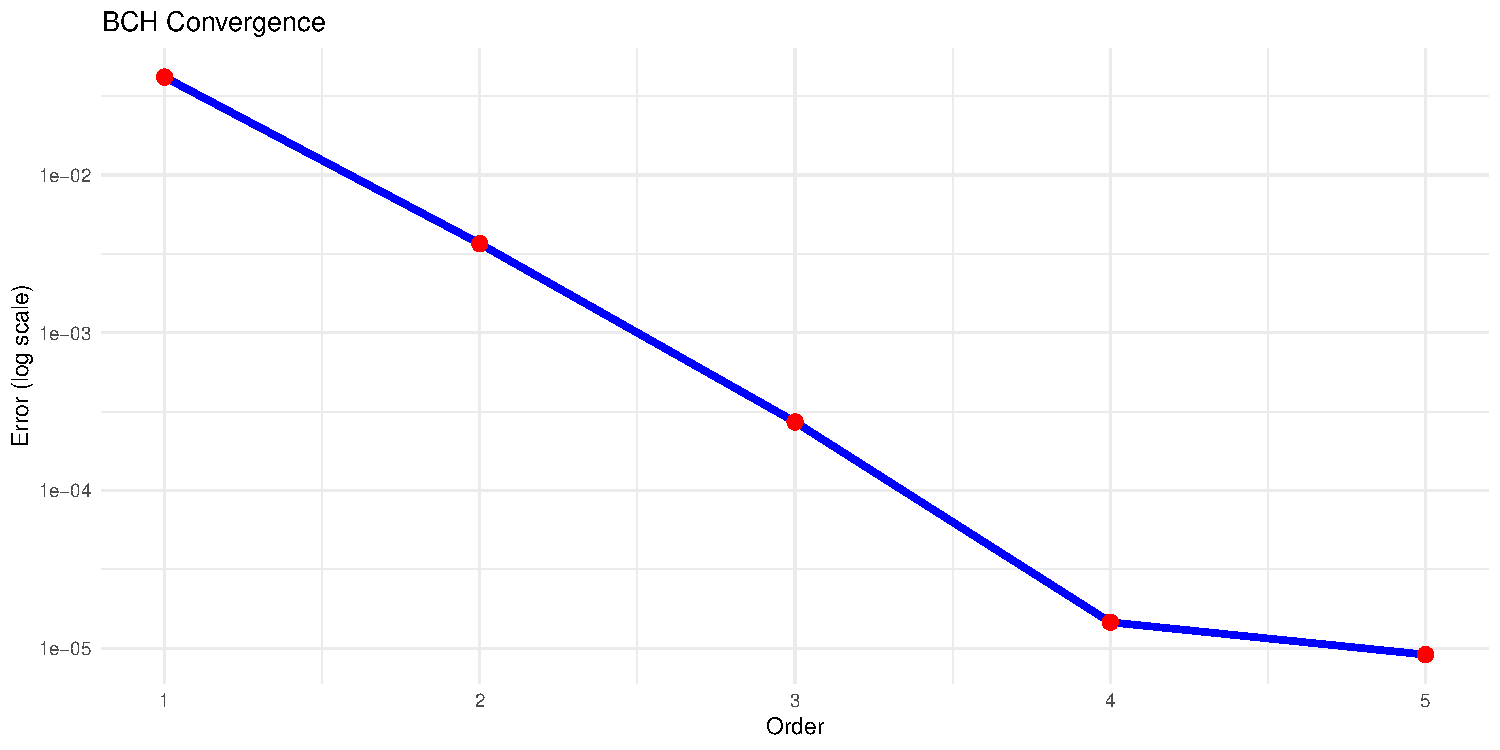
\includegraphics{_main_files/figure-latex/bch-convergence-1} \end{center}

\begin{Shaded}
\begin{Highlighting}[]
\CommentTok{\# Test 1: Convergence by order}
\NormalTok{scale }\OtherTok{\textless{}{-}} \FloatTok{0.05}
\FunctionTok{set.seed}\NormalTok{(}\DecValTok{1000}\NormalTok{)}
\NormalTok{X }\OtherTok{\textless{}{-}}\NormalTok{ scale }\SpecialCharTok{*} \FunctionTok{matrix}\NormalTok{(}\FunctionTok{rnorm}\NormalTok{(}\DecValTok{9}\NormalTok{), }\DecValTok{3}\NormalTok{, }\DecValTok{3}\NormalTok{)}
\NormalTok{Y }\OtherTok{\textless{}{-}}\NormalTok{ scale }\SpecialCharTok{*} \FunctionTok{matrix}\NormalTok{(}\FunctionTok{rnorm}\NormalTok{(}\DecValTok{9}\NormalTok{), }\DecValTok{3}\NormalTok{, }\DecValTok{3}\NormalTok{)}

\NormalTok{direct }\OtherTok{\textless{}{-}} \FunctionTok{expm}\NormalTok{(X) }\SpecialCharTok{\%*\%} \FunctionTok{expm}\NormalTok{(Y)}

\FunctionTok{cat}\NormalTok{(}\FunctionTok{sprintf}\NormalTok{(}\StringTok{"Test matrices: scale = \%.3f}\SpecialCharTok{\textbackslash{}n}\StringTok{"}\NormalTok{, scale))}
\end{Highlighting}
\end{Shaded}

\begin{verbatim}
## Test matrices: scale = 0.050
\end{verbatim}

\begin{Shaded}
\begin{Highlighting}[]
\FunctionTok{cat}\NormalTok{(}\FunctionTok{sprintf}\NormalTok{(}\StringTok{"||X|| = \%.6f, ||Y|| = \%.6f}\SpecialCharTok{\textbackslash{}n}\StringTok{"}\NormalTok{, }\FunctionTok{norm}\NormalTok{(X, }\StringTok{"F"}\NormalTok{), }\FunctionTok{norm}\NormalTok{(Y, }\StringTok{"F"}\NormalTok{)))}
\end{Highlighting}
\end{Shaded}

\begin{verbatim}
## ||X|| = 0.094544, ||Y|| = 0.112094
\end{verbatim}

\begin{Shaded}
\begin{Highlighting}[]
\FunctionTok{cat}\NormalTok{(}\FunctionTok{sprintf}\NormalTok{(}\StringTok{"||[X,Y]|| = \%.6f}\SpecialCharTok{\textbackslash{}n\textbackslash{}n}\StringTok{"}\NormalTok{, }\FunctionTok{norm}\NormalTok{(}\FunctionTok{commutator}\NormalTok{(X, Y), }\StringTok{"F"}\NormalTok{)))}
\end{Highlighting}
\end{Shaded}

\begin{verbatim}
## ||[X,Y]|| = 0.007416
\end{verbatim}

\begin{Shaded}
\begin{Highlighting}[]
\CommentTok{\# Test different orders}
\NormalTok{orders }\OtherTok{\textless{}{-}} \DecValTok{1}\SpecialCharTok{:}\DecValTok{5}
\NormalTok{errors\_by\_order }\OtherTok{\textless{}{-}} \FunctionTok{sapply}\NormalTok{(orders, }\ControlFlowTok{function}\NormalTok{(o) \{}
\NormalTok{  Z }\OtherTok{\textless{}{-}} \FunctionTok{bch\_expansion}\NormalTok{(X, Y, o)}
  \FunctionTok{norm}\NormalTok{(direct }\SpecialCharTok{{-}} \FunctionTok{expm}\NormalTok{(Z), }\StringTok{"F"}\NormalTok{)}
\NormalTok{\})}

\NormalTok{order\_df }\OtherTok{\textless{}{-}} \FunctionTok{data.frame}\NormalTok{(}\AttributeTok{Order =}\NormalTok{ orders, }\AttributeTok{Error =}\NormalTok{ errors\_by\_order)}
\FunctionTok{library}\NormalTok{(ggplot2)}
\NormalTok{p1 }\OtherTok{\textless{}{-}} \FunctionTok{ggplot}\NormalTok{(order\_df, }\FunctionTok{aes}\NormalTok{(}\AttributeTok{x =}\NormalTok{ Order, }\AttributeTok{y =}\NormalTok{ Error)) }\SpecialCharTok{+}
  \FunctionTok{geom\_line}\NormalTok{(}\AttributeTok{color =} \StringTok{"darkblue"}\NormalTok{, }\AttributeTok{size =} \FloatTok{1.5}\NormalTok{) }\SpecialCharTok{+}
  \FunctionTok{geom\_point}\NormalTok{(}\AttributeTok{color =} \StringTok{"red"}\NormalTok{, }\AttributeTok{size =} \DecValTok{4}\NormalTok{) }\SpecialCharTok{+}
  \FunctionTok{geom\_text}\NormalTok{(}\FunctionTok{aes}\NormalTok{(}\AttributeTok{label =} \FunctionTok{sprintf}\NormalTok{(}\StringTok{"\%.2e"}\NormalTok{, Error)), }
            \AttributeTok{vjust =} \SpecialCharTok{{-}}\FloatTok{0.8}\NormalTok{, }\AttributeTok{size =} \FloatTok{3.5}\NormalTok{) }\SpecialCharTok{+}
  \FunctionTok{scale\_y\_log10}\NormalTok{() }\SpecialCharTok{+}
  \FunctionTok{scale\_x\_continuous}\NormalTok{(}\AttributeTok{breaks =} \DecValTok{1}\SpecialCharTok{:}\DecValTok{5}\NormalTok{) }\SpecialCharTok{+}
  \FunctionTok{labs}\NormalTok{(}\AttributeTok{title =} \StringTok{"BCH Formula: Convergence by Order"}\NormalTok{,}
       \AttributeTok{subtitle =} \FunctionTok{sprintf}\NormalTok{(}\StringTok{"Scale = \%.3f"}\NormalTok{, scale),}
       \AttributeTok{x =} \StringTok{"BCH Expansion Order"}\NormalTok{,}
       \AttributeTok{y =} \StringTok{"Error (log scale)"}\NormalTok{) }\SpecialCharTok{+}
  \FunctionTok{theme}\NormalTok{(}\AttributeTok{plot.title =} \FunctionTok{element\_text}\NormalTok{(}\AttributeTok{face =} \StringTok{"bold"}\NormalTok{, }\AttributeTok{size =} \DecValTok{14}\NormalTok{))}

\CommentTok{\# Test 2: Error vs scale}
\NormalTok{scales }\OtherTok{\textless{}{-}} \FunctionTok{seq}\NormalTok{(}\FloatTok{0.01}\NormalTok{, }\FloatTok{0.5}\NormalTok{, }\AttributeTok{by =} \FloatTok{0.01}\NormalTok{)}
\NormalTok{scale\_errors }\OtherTok{\textless{}{-}} \FunctionTok{sapply}\NormalTok{(scales, }\ControlFlowTok{function}\NormalTok{(s) \{}
\NormalTok{  X\_s }\OtherTok{\textless{}{-}}\NormalTok{ s }\SpecialCharTok{*}\NormalTok{ X }\SpecialCharTok{/}\NormalTok{ scale}
\NormalTok{  Y\_s }\OtherTok{\textless{}{-}}\NormalTok{ s }\SpecialCharTok{*}\NormalTok{ Y }\SpecialCharTok{/}\NormalTok{ scale}
\NormalTok{  Z4 }\OtherTok{\textless{}{-}} \FunctionTok{bch\_expansion}\NormalTok{(X\_s, Y\_s, }\AttributeTok{order =} \DecValTok{4}\NormalTok{)}
  \FunctionTok{norm}\NormalTok{(}\FunctionTok{expm}\NormalTok{(X\_s) }\SpecialCharTok{\%*\%} \FunctionTok{expm}\NormalTok{(Y\_s) }\SpecialCharTok{{-}} \FunctionTok{expm}\NormalTok{(Z4), }\StringTok{"F"}\NormalTok{)}
\NormalTok{\})}

\NormalTok{scale\_df }\OtherTok{\textless{}{-}} \FunctionTok{data.frame}\NormalTok{(}\AttributeTok{Scale =}\NormalTok{ scales, }\AttributeTok{Error =}\NormalTok{ scale\_errors)}

\NormalTok{p2 }\OtherTok{\textless{}{-}} \FunctionTok{ggplot}\NormalTok{(scale\_df, }\FunctionTok{aes}\NormalTok{(}\AttributeTok{x =}\NormalTok{ Scale, }\AttributeTok{y =}\NormalTok{ Error)) }\SpecialCharTok{+}
  \FunctionTok{geom\_line}\NormalTok{(}\AttributeTok{color =} \StringTok{"darkgreen"}\NormalTok{, }\AttributeTok{size =} \FloatTok{1.2}\NormalTok{) }\SpecialCharTok{+}
  \FunctionTok{geom\_point}\NormalTok{(}\FunctionTok{aes}\NormalTok{(}\AttributeTok{color =}\NormalTok{ Error), }\AttributeTok{size =} \DecValTok{2}\NormalTok{) }\SpecialCharTok{+}
  \FunctionTok{scale\_y\_log10}\NormalTok{() }\SpecialCharTok{+}
  \FunctionTok{scale\_color\_gradient}\NormalTok{(}\AttributeTok{low =} \StringTok{"green"}\NormalTok{, }\AttributeTok{high =} \StringTok{"red"}\NormalTok{, }\AttributeTok{guide =} \StringTok{"none"}\NormalTok{) }\SpecialCharTok{+}
  \FunctionTok{geom\_vline}\NormalTok{(}\AttributeTok{xintercept =} \FloatTok{0.1}\NormalTok{, }\AttributeTok{linetype =} \StringTok{"dashed"}\NormalTok{, }\AttributeTok{alpha =} \FloatTok{0.5}\NormalTok{) }\SpecialCharTok{+}
  \FunctionTok{annotate}\NormalTok{(}\StringTok{"text"}\NormalTok{, }\AttributeTok{x =} \FloatTok{0.15}\NormalTok{, }\AttributeTok{y =} \FunctionTok{max}\NormalTok{(scale\_errors)}\SpecialCharTok{/}\DecValTok{10}\NormalTok{, }
           \AttributeTok{label =} \StringTok{"Convergence}\SpecialCharTok{\textbackslash{}n}\StringTok{breaks down →"}\NormalTok{, }\AttributeTok{size =} \DecValTok{3}\NormalTok{) }\SpecialCharTok{+}
  \FunctionTok{labs}\NormalTok{(}\AttributeTok{title =} \StringTok{"BCH Formula: Error vs Matrix Scale"}\NormalTok{,}
       \AttributeTok{subtitle =} \StringTok{"Order 4 expansion"}\NormalTok{,}
       \AttributeTok{x =} \StringTok{"Scale Factor"}\NormalTok{,}
       \AttributeTok{y =} \StringTok{"Error (log scale)"}\NormalTok{) }\SpecialCharTok{+}
  \FunctionTok{theme}\NormalTok{(}\AttributeTok{plot.title =} \FunctionTok{element\_text}\NormalTok{(}\AttributeTok{face =} \StringTok{"bold"}\NormalTok{, }\AttributeTok{size =} \DecValTok{14}\NormalTok{))}

\FunctionTok{grid.arrange}\NormalTok{(p1, p2, }\AttributeTok{ncol =} \DecValTok{1}\NormalTok{)}
\end{Highlighting}
\end{Shaded}

\begin{center}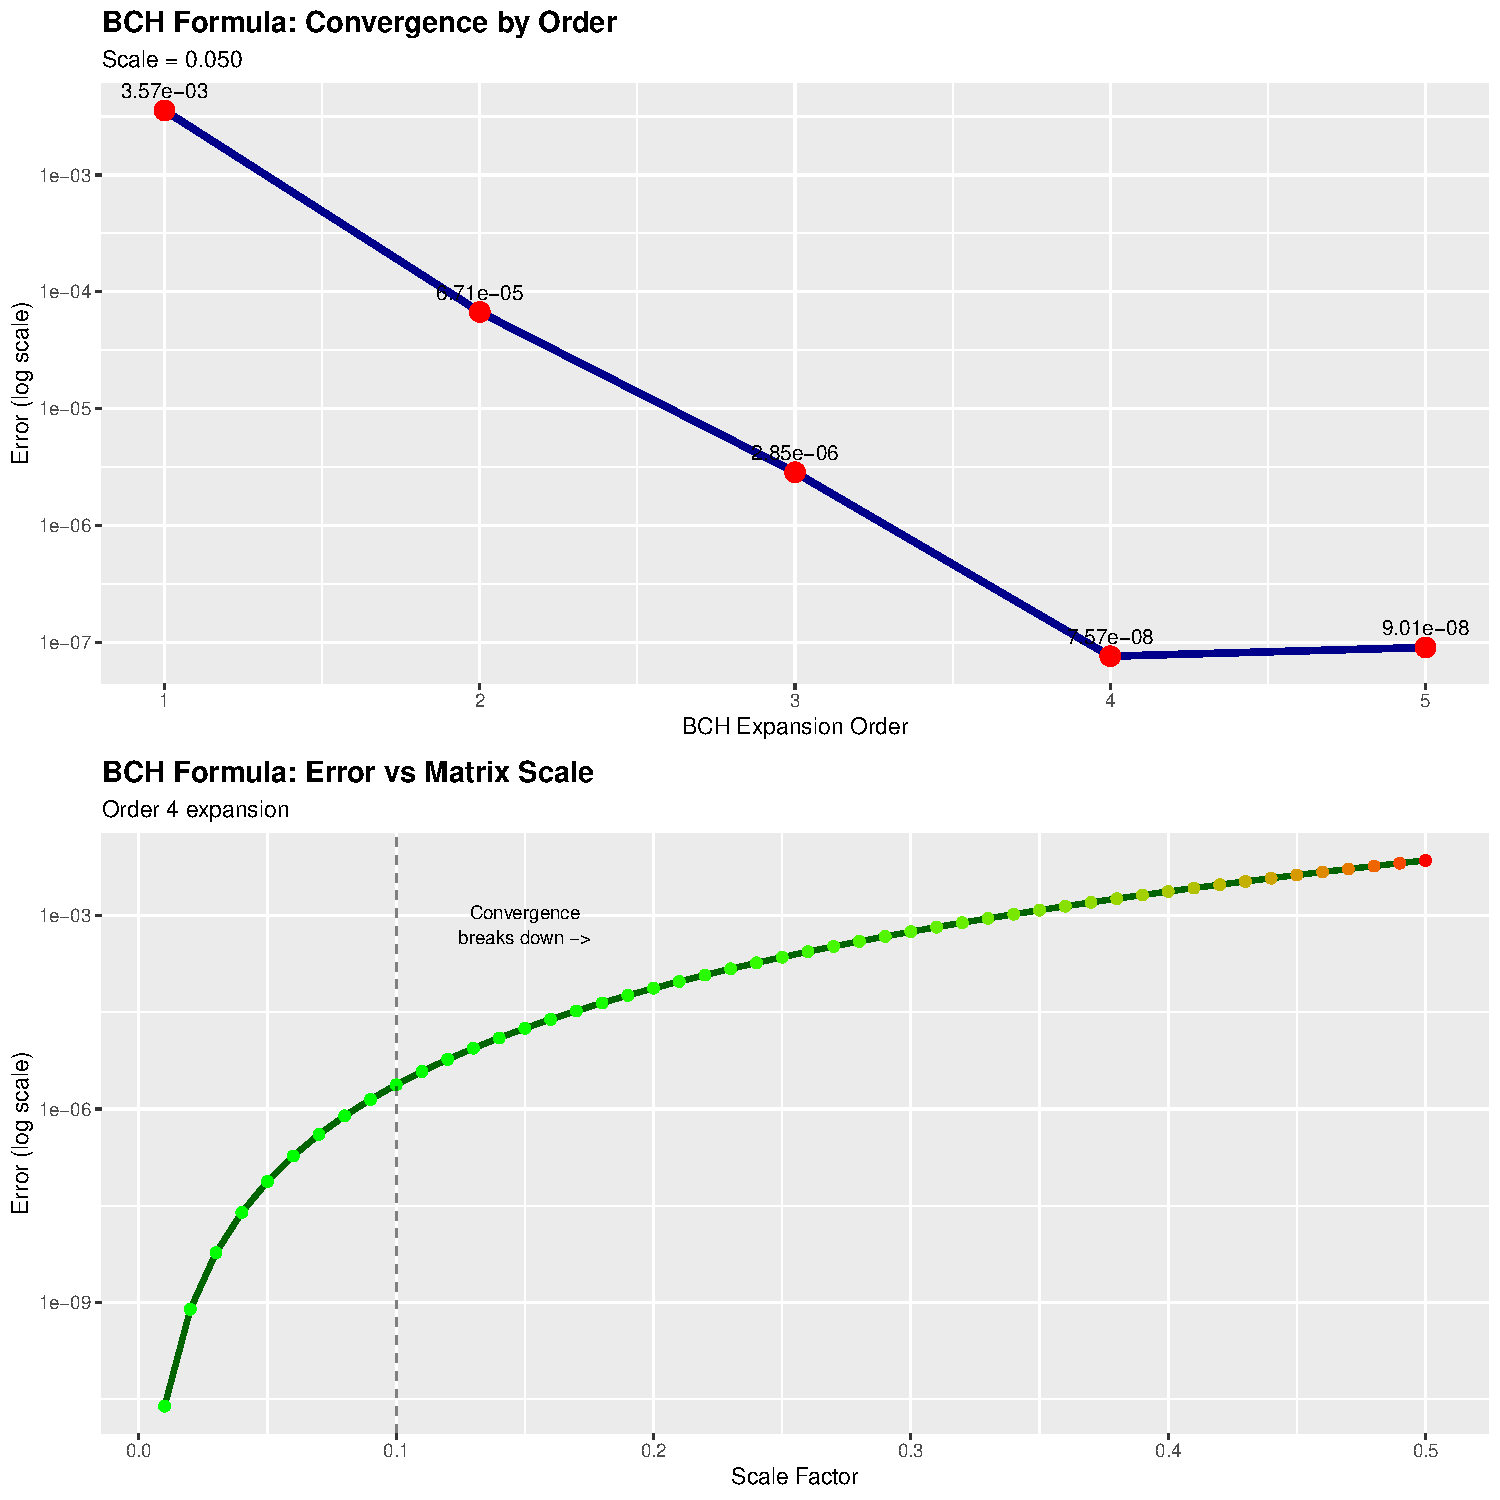
\includegraphics{_main_files/figure-latex/bch-convergence-detailed-1} \end{center}

\begin{Shaded}
\begin{Highlighting}[]
\CommentTok{\# Find approximate convergence radius}
\NormalTok{conv\_threshold }\OtherTok{\textless{}{-}} \FloatTok{0.01}
\NormalTok{conv\_scale }\OtherTok{\textless{}{-}} \FunctionTok{max}\NormalTok{(scales[scale\_errors }\SpecialCharTok{\textless{}}\NormalTok{ conv\_threshold])}
\FunctionTok{cat}\NormalTok{(}\FunctionTok{sprintf}\NormalTok{(}\StringTok{"}\SpecialCharTok{\textbackslash{}n}\StringTok{Approximate convergence radius: scale \textless{} \%.3f}\SpecialCharTok{\textbackslash{}n}\StringTok{"}\NormalTok{, conv\_scale))}
\end{Highlighting}
\end{Shaded}

\begin{verbatim}
## 
## Approximate convergence radius: scale < 0.500
\end{verbatim}

\begin{Shaded}
\begin{Highlighting}[]
\NormalTok{comparison\_data }\OtherTok{\textless{}{-}} \FunctionTok{data.frame}\NormalTok{(}
  \AttributeTok{Scale =} \FunctionTok{c}\NormalTok{(}\FloatTok{0.01}\NormalTok{, }\FloatTok{0.05}\NormalTok{, }\FloatTok{0.1}\NormalTok{, }\FloatTok{0.2}\NormalTok{, }\FloatTok{0.5}\NormalTok{),}
  \AttributeTok{Order\_2 =} \ConstantTok{NA}\NormalTok{,}
  \AttributeTok{Order\_3 =} \ConstantTok{NA}\NormalTok{,}
  \AttributeTok{Order\_4 =} \ConstantTok{NA}\NormalTok{,}
  \AttributeTok{Order\_5 =} \ConstantTok{NA}
\NormalTok{)}

\ControlFlowTok{for}\NormalTok{ (i }\ControlFlowTok{in} \DecValTok{1}\SpecialCharTok{:}\FunctionTok{nrow}\NormalTok{(comparison\_data)) \{}
\NormalTok{  s }\OtherTok{\textless{}{-}}\NormalTok{ comparison\_data}\SpecialCharTok{$}\NormalTok{Scale[i]}
\NormalTok{  X\_s }\OtherTok{\textless{}{-}}\NormalTok{ s }\SpecialCharTok{*}\NormalTok{ X }\SpecialCharTok{/}\NormalTok{ scale}
\NormalTok{  Y\_s }\OtherTok{\textless{}{-}}\NormalTok{ s }\SpecialCharTok{*}\NormalTok{ Y }\SpecialCharTok{/}\NormalTok{ scale}
\NormalTok{  direct\_s }\OtherTok{\textless{}{-}} \FunctionTok{expm}\NormalTok{(X\_s) }\SpecialCharTok{\%*\%} \FunctionTok{expm}\NormalTok{(Y\_s)}
  
  \ControlFlowTok{for}\NormalTok{ (o }\ControlFlowTok{in} \DecValTok{2}\SpecialCharTok{:}\DecValTok{5}\NormalTok{) \{}
\NormalTok{    Z }\OtherTok{\textless{}{-}} \FunctionTok{bch\_expansion}\NormalTok{(X\_s, Y\_s, }\AttributeTok{order =}\NormalTok{ o)}
\NormalTok{    comparison\_data[i, o] }\OtherTok{\textless{}{-}} \FunctionTok{norm}\NormalTok{(direct\_s }\SpecialCharTok{{-}} \FunctionTok{expm}\NormalTok{(Z), }\StringTok{"F"}\NormalTok{)}
\NormalTok{  \}}
\NormalTok{\}}

\FunctionTok{kable}\NormalTok{(comparison\_data,}
      \AttributeTok{digits =} \DecValTok{10}\NormalTok{,}
      \AttributeTok{caption =} \StringTok{"BCH Formula Accuracy: Error vs Scale and Order"}\NormalTok{,}
      \AttributeTok{col.names =} \FunctionTok{c}\NormalTok{(}\StringTok{"Scale"}\NormalTok{, }\StringTok{"Order 2"}\NormalTok{, }\StringTok{"Order 3"}\NormalTok{, }\StringTok{"Order 4"}\NormalTok{, }\StringTok{"Order 5"}\NormalTok{)) }\SpecialCharTok{\%\textgreater{}\%}
  \FunctionTok{kable\_styling}\NormalTok{(}\AttributeTok{bootstrap\_options =} \FunctionTok{c}\NormalTok{(}\StringTok{"striped"}\NormalTok{, }\StringTok{"hover"}\NormalTok{)) }\SpecialCharTok{\%\textgreater{}\%}
  \FunctionTok{column\_spec}\NormalTok{(}\DecValTok{1}\NormalTok{, }\AttributeTok{bold =} \ConstantTok{TRUE}\NormalTok{) }\SpecialCharTok{\%\textgreater{}\%}
  \FunctionTok{row\_spec}\NormalTok{(}\FunctionTok{which}\NormalTok{(comparison\_data}\SpecialCharTok{$}\NormalTok{Scale }\SpecialCharTok{\textless{}=} \FloatTok{0.1}\NormalTok{), }\AttributeTok{background =} \StringTok{"\#e6f9e6"}\NormalTok{)}
\end{Highlighting}
\end{Shaded}

\label{tab:bch-comparison-table}BCH Formula Accuracy: Error vs Scale and Order

Scale

Order 2

Order 3

Order 4

Order 5

0.01

0.0000005550

0.0000000047

0.0000000000

0.0000000000

0.05

0.0000670943

0.0000028463

0.0000000757

0.0000000901

0.10

0.0005176194

0.0000439017

0.0000023792

0.0000028287

0.20

0.0039195236

0.0006558386

0.0000745327

0.0000884600

0.50

0.0570375336

0.0216619394

0.0071690943

0.0083980888

\textbf{Key Observations}: BCH formula is highly accurate for \(\|X\|, \|Y\| < 0.1\). Higher orders provide diminishing returns beyond order 4 for small matrices. But breaks down rapidly for larger matrices. This confirms that ``sufficiently small'' means roughly \(||X||, ||Y|| \lesssim 0.2\)

\section{SO(3) Rotation Group}\label{so3-rotation-group}

\subsection{Mathematical Background}\label{mathematical-background}

\(SO(3) = \{R \in M_3(\mathbb{R}) : R^TR = I, \det(R) = 1\}\) is the group of rotations in 3D space.

Its Lie algebra is:
\[\mathfrak{so}(3) = \{X \in M_3(\mathbb{R}) : X^T = -X\}\]

Any skew-symmetric matrix can be written as:
\[X = \begin{pmatrix} 0 & -c & b \\ c & 0 & -a \\ -b & a & 0 \end{pmatrix}\]

corresponding to the axis vector \((a, b, c)^T\).

\begin{Shaded}
\begin{Highlighting}[]
\NormalTok{skew\_symmetric }\OtherTok{\textless{}{-}} \ControlFlowTok{function}\NormalTok{(v) \{}
  \FunctionTok{matrix}\NormalTok{(}\FunctionTok{c}\NormalTok{(}\DecValTok{0}\NormalTok{, v[}\DecValTok{3}\NormalTok{], }\SpecialCharTok{{-}}\NormalTok{v[}\DecValTok{2}\NormalTok{], }\SpecialCharTok{{-}}\NormalTok{v[}\DecValTok{3}\NormalTok{], }\DecValTok{0}\NormalTok{, v[}\DecValTok{1}\NormalTok{], v[}\DecValTok{2}\NormalTok{], }\SpecialCharTok{{-}}\NormalTok{v[}\DecValTok{1}\NormalTok{], }\DecValTok{0}\NormalTok{), }\DecValTok{3}\NormalTok{, }\DecValTok{3}\NormalTok{, }\AttributeTok{byrow =} \ConstantTok{TRUE}\NormalTok{)}
\NormalTok{\}}

\FunctionTok{set.seed}\NormalTok{(}\DecValTok{789}\NormalTok{)}
\NormalTok{v }\OtherTok{\textless{}{-}} \FunctionTok{rnorm}\NormalTok{(}\DecValTok{3}\NormalTok{)}
\NormalTok{X }\OtherTok{\textless{}{-}} \FunctionTok{skew\_symmetric}\NormalTok{(v)}
\NormalTok{R }\OtherTok{\textless{}{-}} \FunctionTok{expm}\NormalTok{(X)}

\NormalTok{so3\_props }\OtherTok{\textless{}{-}} \FunctionTok{data.frame}\NormalTok{(}
  \AttributeTok{Property =} \FunctionTok{c}\NormalTok{(}\StringTok{"R\^{}T·R = I"}\NormalTok{, }\StringTok{"det(R) = 1"}\NormalTok{, }\StringTok{"X is skew{-}symmetric"}\NormalTok{),}
  \AttributeTok{Verified =} \FunctionTok{c}\NormalTok{(}
    \FunctionTok{max}\NormalTok{(}\FunctionTok{abs}\NormalTok{(}\FunctionTok{t}\NormalTok{(R) }\SpecialCharTok{\%*\%}\NormalTok{ R }\SpecialCharTok{{-}} \FunctionTok{diag}\NormalTok{(}\DecValTok{3}\NormalTok{))) }\SpecialCharTok{\textless{}} \FloatTok{1e{-}10}\NormalTok{,}
    \FunctionTok{abs}\NormalTok{(}\FunctionTok{det}\NormalTok{(R) }\SpecialCharTok{{-}} \DecValTok{1}\NormalTok{) }\SpecialCharTok{\textless{}} \FloatTok{1e{-}10}\NormalTok{,}
    \FunctionTok{max}\NormalTok{(}\FunctionTok{abs}\NormalTok{(X }\SpecialCharTok{+} \FunctionTok{t}\NormalTok{(X))) }\SpecialCharTok{\textless{}} \FloatTok{1e{-}14}
\NormalTok{  )}
\NormalTok{)}

\FunctionTok{kable}\NormalTok{(so3\_props, }\AttributeTok{caption =} \StringTok{"SO(3) Properties"}\NormalTok{) }\SpecialCharTok{\%\textgreater{}\%}
  \FunctionTok{kable\_styling}\NormalTok{() }\SpecialCharTok{\%\textgreater{}\%}
  \FunctionTok{column\_spec}\NormalTok{(}\DecValTok{2}\NormalTok{, }\AttributeTok{bold =} \ConstantTok{TRUE}\NormalTok{, }\AttributeTok{color =} \FunctionTok{ifelse}\NormalTok{(so3\_props}\SpecialCharTok{$}\NormalTok{Verified, }\StringTok{"green"}\NormalTok{, }\StringTok{"red"}\NormalTok{))}
\end{Highlighting}
\end{Shaded}

\label{tab:so3-implementation}SO(3) Properties

Property

Verified

R\^{}T·R = I

TRUE

det(R) = 1

TRUE

X is skew-symmetric

TRUE

\begin{Shaded}
\begin{Highlighting}[]
\NormalTok{axis }\OtherTok{\textless{}{-}} \FunctionTok{c}\NormalTok{(}\DecValTok{1}\NormalTok{, }\DecValTok{1}\NormalTok{, }\DecValTok{1}\NormalTok{) }\SpecialCharTok{/} \FunctionTok{sqrt}\NormalTok{(}\DecValTok{3}\NormalTok{)}
\NormalTok{X }\OtherTok{\textless{}{-}} \FunctionTok{skew\_symmetric}\NormalTok{(axis)}
\NormalTok{v0 }\OtherTok{\textless{}{-}} \FunctionTok{c}\NormalTok{(}\DecValTok{1}\NormalTok{, }\DecValTok{0}\NormalTok{, }\DecValTok{0}\NormalTok{)}
\NormalTok{t\_vals }\OtherTok{\textless{}{-}} \FunctionTok{seq}\NormalTok{(}\DecValTok{0}\NormalTok{, }\DecValTok{2}\SpecialCharTok{*}\NormalTok{pi, }\AttributeTok{length.out =} \DecValTok{100}\NormalTok{)}
\NormalTok{path }\OtherTok{\textless{}{-}} \FunctionTok{t}\NormalTok{(}\FunctionTok{sapply}\NormalTok{(t\_vals, }\ControlFlowTok{function}\NormalTok{(t) }\FunctionTok{as.vector}\NormalTok{(}\FunctionTok{expm}\NormalTok{(t }\SpecialCharTok{*}\NormalTok{ X) }\SpecialCharTok{\%*\%}\NormalTok{ v0)))}

\NormalTok{theta }\OtherTok{\textless{}{-}} \FunctionTok{seq}\NormalTok{(}\DecValTok{0}\NormalTok{, }\DecValTok{2}\SpecialCharTok{*}\NormalTok{pi, }\AttributeTok{length.out =} \DecValTok{50}\NormalTok{)}
\NormalTok{phi }\OtherTok{\textless{}{-}} \FunctionTok{seq}\NormalTok{(}\DecValTok{0}\NormalTok{, pi, }\AttributeTok{length.out =} \DecValTok{50}\NormalTok{)}
\NormalTok{grid }\OtherTok{\textless{}{-}} \FunctionTok{expand.grid}\NormalTok{(}\AttributeTok{theta =}\NormalTok{ theta, }\AttributeTok{phi =}\NormalTok{ phi)}
\NormalTok{sphere\_x }\OtherTok{\textless{}{-}} \FunctionTok{matrix}\NormalTok{(}\FunctionTok{sin}\NormalTok{(grid}\SpecialCharTok{$}\NormalTok{phi) }\SpecialCharTok{*} \FunctionTok{cos}\NormalTok{(grid}\SpecialCharTok{$}\NormalTok{theta), }\DecValTok{50}\NormalTok{, }\DecValTok{50}\NormalTok{)}
\NormalTok{sphere\_y }\OtherTok{\textless{}{-}} \FunctionTok{matrix}\NormalTok{(}\FunctionTok{sin}\NormalTok{(grid}\SpecialCharTok{$}\NormalTok{phi) }\SpecialCharTok{*} \FunctionTok{sin}\NormalTok{(grid}\SpecialCharTok{$}\NormalTok{theta), }\DecValTok{50}\NormalTok{, }\DecValTok{50}\NormalTok{)}
\NormalTok{sphere\_z }\OtherTok{\textless{}{-}} \FunctionTok{matrix}\NormalTok{(}\FunctionTok{cos}\NormalTok{(grid}\SpecialCharTok{$}\NormalTok{phi), }\DecValTok{50}\NormalTok{, }\DecValTok{50}\NormalTok{)}

\FunctionTok{plot\_ly}\NormalTok{() }\SpecialCharTok{\%\textgreater{}\%}
  \FunctionTok{add\_surface}\NormalTok{(}\AttributeTok{x =}\NormalTok{ sphere\_x, }\AttributeTok{y =}\NormalTok{ sphere\_y, }\AttributeTok{z =}\NormalTok{ sphere\_z, }
              \AttributeTok{opacity =} \FloatTok{0.2}\NormalTok{, }\AttributeTok{showscale =} \ConstantTok{FALSE}\NormalTok{) }\SpecialCharTok{\%\textgreater{}\%}
  \FunctionTok{add\_trace}\NormalTok{(}\AttributeTok{type =} \StringTok{"scatter3d"}\NormalTok{, }\AttributeTok{mode =} \StringTok{"lines"}\NormalTok{,}
            \AttributeTok{x =}\NormalTok{ path[,}\DecValTok{1}\NormalTok{], }\AttributeTok{y =}\NormalTok{ path[,}\DecValTok{2}\NormalTok{], }\AttributeTok{z =}\NormalTok{ path[,}\DecValTok{3}\NormalTok{],}
            \AttributeTok{line =} \FunctionTok{list}\NormalTok{(}\AttributeTok{color =} \StringTok{"red"}\NormalTok{, }\AttributeTok{width =} \DecValTok{5}\NormalTok{)) }\SpecialCharTok{\%\textgreater{}\%}
  \FunctionTok{layout}\NormalTok{(}\AttributeTok{title =} \StringTok{"SO(3) Rotation on Unit Sphere"}\NormalTok{,}
         \AttributeTok{scene =} \FunctionTok{list}\NormalTok{(}\AttributeTok{aspectmode =} \StringTok{"cube"}\NormalTok{))}
\end{Highlighting}
\end{Shaded}

\begin{center}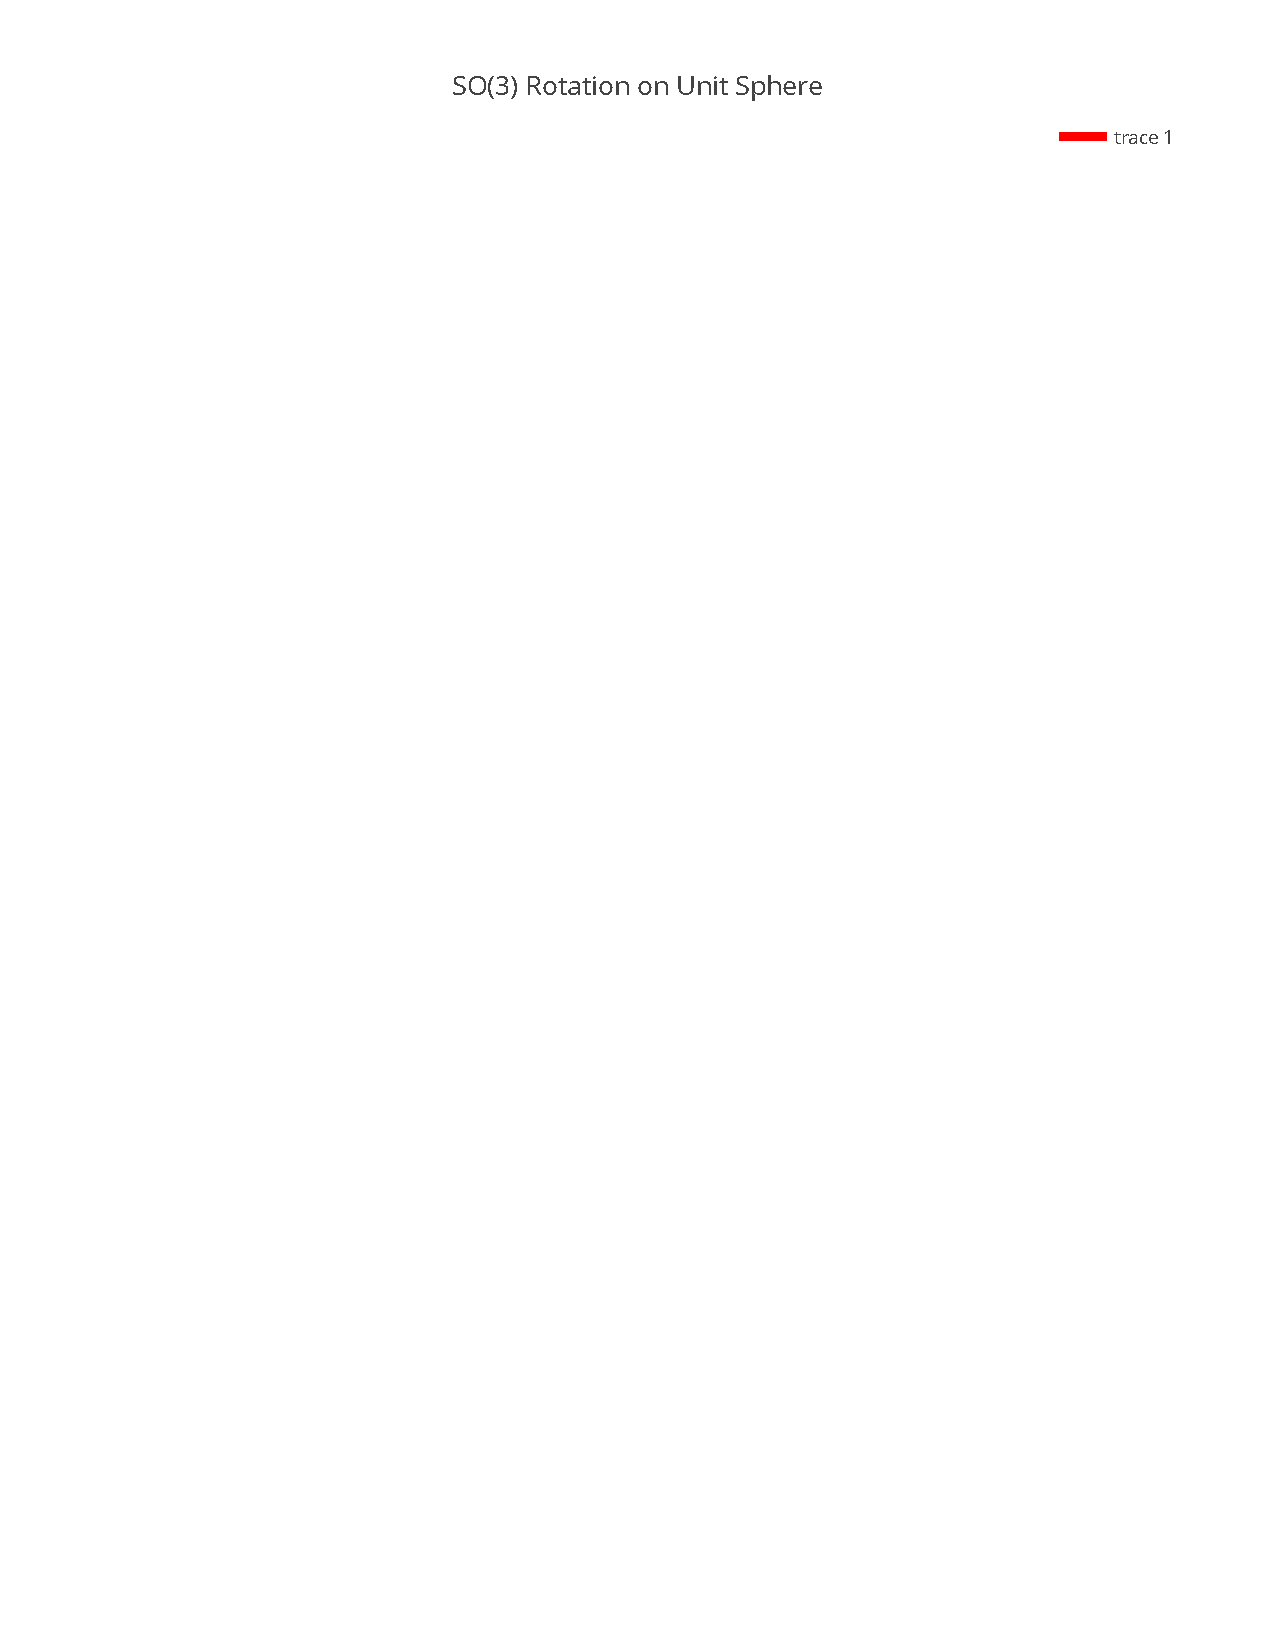
\includegraphics{_main_files/figure-latex/so3-visualization-1} \end{center}

\section{SU(2) Special Unitary Group}\label{su2-special-unitary-group}

\begin{Shaded}
\begin{Highlighting}[]
\NormalTok{pauli\_matrices }\OtherTok{\textless{}{-}} \ControlFlowTok{function}\NormalTok{() \{}
  \FunctionTok{list}\NormalTok{(}\AttributeTok{x =} \FunctionTok{matrix}\NormalTok{(}\FunctionTok{c}\NormalTok{(}\DecValTok{0}\NormalTok{, }\DecValTok{1}\NormalTok{, }\DecValTok{1}\NormalTok{, }\DecValTok{0}\NormalTok{), }\DecValTok{2}\NormalTok{, }\DecValTok{2}\NormalTok{),}
       \AttributeTok{y =} \FunctionTok{matrix}\NormalTok{(}\FunctionTok{c}\NormalTok{(}\DecValTok{0}\NormalTok{, }\SpecialCharTok{{-}}\DecValTok{1}\DataTypeTok{i}\NormalTok{, }\DecValTok{1}\DataTypeTok{i}\NormalTok{, }\DecValTok{0}\NormalTok{), }\DecValTok{2}\NormalTok{, }\DecValTok{2}\NormalTok{),}
       \AttributeTok{z =} \FunctionTok{matrix}\NormalTok{(}\FunctionTok{c}\NormalTok{(}\DecValTok{1}\NormalTok{, }\DecValTok{0}\NormalTok{, }\DecValTok{0}\NormalTok{, }\SpecialCharTok{{-}}\DecValTok{1}\NormalTok{), }\DecValTok{2}\NormalTok{, }\DecValTok{2}\NormalTok{))}
\NormalTok{\}}

\NormalTok{sigma }\OtherTok{\textless{}{-}} \FunctionTok{pauli\_matrices}\NormalTok{()}
\NormalTok{X\_su2 }\OtherTok{\textless{}{-}} \DecValTok{1}\DataTypeTok{i} \SpecialCharTok{*}\NormalTok{ sigma}\SpecialCharTok{$}\NormalTok{x }\SpecialCharTok{/} \DecValTok{2}
\NormalTok{exp\_2pi }\OtherTok{\textless{}{-}} \FunctionTok{expm}\NormalTok{(}\DecValTok{2}\SpecialCharTok{*}\NormalTok{pi}\SpecialCharTok{*}\NormalTok{X\_su2)}
\NormalTok{exp\_4pi }\OtherTok{\textless{}{-}} \FunctionTok{expm}\NormalTok{(}\DecValTok{4}\SpecialCharTok{*}\NormalTok{pi}\SpecialCharTok{*}\NormalTok{X\_su2)}

\NormalTok{su2\_props }\OtherTok{\textless{}{-}} \FunctionTok{data.frame}\NormalTok{(}
  \AttributeTok{Property =} \FunctionTok{c}\NormalTok{(}\StringTok{"X is traceless"}\NormalTok{, }\StringTok{"X is anti{-}Hermitian"}\NormalTok{, }
               \StringTok{"exp(2π·X) = {-}I"}\NormalTok{, }\StringTok{"exp(4π·X) = I"}\NormalTok{),}
  \AttributeTok{Verified =} \FunctionTok{c}\NormalTok{(}
    \FunctionTok{abs}\NormalTok{(}\FunctionTok{sum}\NormalTok{(}\FunctionTok{diag}\NormalTok{(X\_su2))) }\SpecialCharTok{\textless{}} \FloatTok{1e{-}14}\NormalTok{,}
    \FunctionTok{max}\NormalTok{(}\FunctionTok{abs}\NormalTok{(X\_su2 }\SpecialCharTok{+} \FunctionTok{Conj}\NormalTok{(}\FunctionTok{t}\NormalTok{(X\_su2)))) }\SpecialCharTok{\textless{}} \FloatTok{1e{-}14}\NormalTok{,}
    \FunctionTok{max}\NormalTok{(}\FunctionTok{abs}\NormalTok{(exp\_2pi }\SpecialCharTok{+} \FunctionTok{diag}\NormalTok{(}\DecValTok{2}\NormalTok{))) }\SpecialCharTok{\textless{}} \FloatTok{1e{-}10}\NormalTok{,}
    \FunctionTok{max}\NormalTok{(}\FunctionTok{abs}\NormalTok{(exp\_4pi }\SpecialCharTok{{-}} \FunctionTok{diag}\NormalTok{(}\DecValTok{2}\NormalTok{))) }\SpecialCharTok{\textless{}} \FloatTok{1e{-}10}
\NormalTok{  )}
\NormalTok{)}

\FunctionTok{kable}\NormalTok{(su2\_props, }\AttributeTok{caption =} \StringTok{"SU(2) Double Cover"}\NormalTok{) }\SpecialCharTok{\%\textgreater{}\%}
  \FunctionTok{kable\_styling}\NormalTok{() }\SpecialCharTok{\%\textgreater{}\%}
  \FunctionTok{column\_spec}\NormalTok{(}\DecValTok{2}\NormalTok{, }\AttributeTok{bold =} \ConstantTok{TRUE}\NormalTok{, }\AttributeTok{color =} \FunctionTok{ifelse}\NormalTok{(su2\_props}\SpecialCharTok{$}\NormalTok{Verified, }\StringTok{"green"}\NormalTok{, }\StringTok{"red"}\NormalTok{))}
\end{Highlighting}
\end{Shaded}

\label{tab:pauli-matrices}SU(2) Double Cover

Property

Verified

X is traceless

TRUE

X is anti-Hermitian

TRUE

exp(2π·X) = -I

TRUE

exp(4π·X) = I

TRUE

\begin{Shaded}
\begin{Highlighting}[]
\NormalTok{t\_vals }\OtherTok{\textless{}{-}} \FunctionTok{seq}\NormalTok{(}\DecValTok{0}\NormalTok{, }\DecValTok{4}\SpecialCharTok{*}\NormalTok{pi, }\AttributeTok{length.out =} \DecValTok{200}\NormalTok{)}

\DocumentationTok{\#\# Compute determinants {-} use product of eigenvalues for complex matrices}
\NormalTok{dets }\OtherTok{\textless{}{-}} \FunctionTok{sapply}\NormalTok{(t\_vals, }\ControlFlowTok{function}\NormalTok{(t) \{}
\NormalTok{  M }\OtherTok{\textless{}{-}} \FunctionTok{expm}\NormalTok{(t}\SpecialCharTok{*}\NormalTok{X\_su2)}
  \FunctionTok{prod}\NormalTok{(}\FunctionTok{eigen}\NormalTok{(M, }\AttributeTok{only.values =} \ConstantTok{TRUE}\NormalTok{)}\SpecialCharTok{$}\NormalTok{values)}
\NormalTok{\})}

\FunctionTok{ggplot}\NormalTok{(}\FunctionTok{data.frame}\NormalTok{(}\AttributeTok{t =}\NormalTok{ t\_vals}\SpecialCharTok{/}\NormalTok{pi, }\AttributeTok{real =} \FunctionTok{Re}\NormalTok{(dets), }\AttributeTok{imag =} \FunctionTok{Im}\NormalTok{(dets))) }\SpecialCharTok{+}
  \FunctionTok{geom\_line}\NormalTok{(}\FunctionTok{aes}\NormalTok{(}\AttributeTok{x =}\NormalTok{ t, }\AttributeTok{y =}\NormalTok{ real, }\AttributeTok{color =} \StringTok{"Real"}\NormalTok{), }\AttributeTok{size =} \FloatTok{1.2}\NormalTok{) }\SpecialCharTok{+}
  \FunctionTok{geom\_line}\NormalTok{(}\FunctionTok{aes}\NormalTok{(}\AttributeTok{x =}\NormalTok{ t, }\AttributeTok{y =}\NormalTok{ imag, }\AttributeTok{color =} \StringTok{"Imag"}\NormalTok{), }\AttributeTok{size =} \FloatTok{1.2}\NormalTok{) }\SpecialCharTok{+}
  \FunctionTok{geom\_hline}\NormalTok{(}\AttributeTok{yintercept =} \FunctionTok{c}\NormalTok{(}\SpecialCharTok{{-}}\DecValTok{1}\NormalTok{, }\DecValTok{1}\NormalTok{), }\AttributeTok{linetype =} \StringTok{"dashed"}\NormalTok{, }\AttributeTok{alpha =} \FloatTok{0.5}\NormalTok{) }\SpecialCharTok{+}
  \FunctionTok{geom\_vline}\NormalTok{(}\AttributeTok{xintercept =} \FunctionTok{c}\NormalTok{(}\DecValTok{2}\NormalTok{, }\DecValTok{4}\NormalTok{), }\AttributeTok{linetype =} \StringTok{"dashed"}\NormalTok{) }\SpecialCharTok{+}
  \FunctionTok{labs}\NormalTok{(}\AttributeTok{title =} \StringTok{"SU(2): det(exp(tX))"}\NormalTok{, }\AttributeTok{x =} \StringTok{"t/π"}\NormalTok{, }\AttributeTok{y =} \StringTok{"Determinant"}\NormalTok{) }\SpecialCharTok{+}
  \FunctionTok{theme\_minimal}\NormalTok{()}
\end{Highlighting}
\end{Shaded}

\begin{center}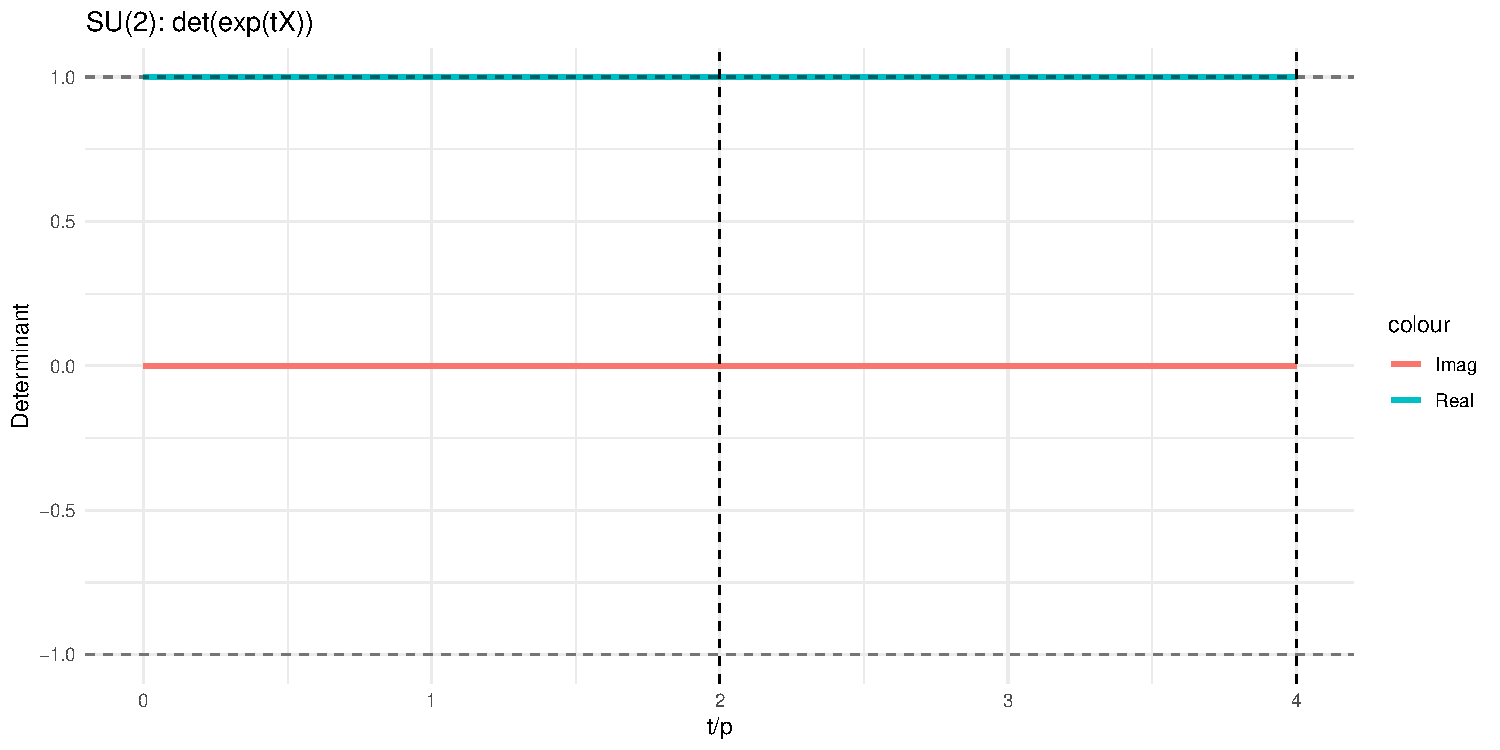
\includegraphics{_main_files/figure-latex/su2-evolution-1} \end{center}

\section{Quantum Rotation Operators}\label{quantum-rotation-operators}

\begin{Shaded}
\begin{Highlighting}[]
\NormalTok{rotation\_operator }\OtherTok{\textless{}{-}} \ControlFlowTok{function}\NormalTok{(theta, n) \{}
\NormalTok{  n }\OtherTok{\textless{}{-}}\NormalTok{ n }\SpecialCharTok{/} \FunctionTok{sqrt}\NormalTok{(}\FunctionTok{sum}\NormalTok{(n}\SpecialCharTok{\^{}}\DecValTok{2}\NormalTok{))}
\NormalTok{  sigma }\OtherTok{\textless{}{-}} \FunctionTok{pauli\_matrices}\NormalTok{()}
\NormalTok{  J\_dot\_n }\OtherTok{\textless{}{-}}\NormalTok{ (n[}\DecValTok{1}\NormalTok{]}\SpecialCharTok{*}\NormalTok{sigma}\SpecialCharTok{$}\NormalTok{x }\SpecialCharTok{+}\NormalTok{ n[}\DecValTok{2}\NormalTok{]}\SpecialCharTok{*}\NormalTok{sigma}\SpecialCharTok{$}\NormalTok{y }\SpecialCharTok{+}\NormalTok{ n[}\DecValTok{3}\NormalTok{]}\SpecialCharTok{*}\NormalTok{sigma}\SpecialCharTok{$}\NormalTok{z) }\SpecialCharTok{/} \DecValTok{2}
  \FunctionTok{expm}\NormalTok{(}\SpecialCharTok{{-}}\DecValTok{1}\DataTypeTok{i} \SpecialCharTok{*}\NormalTok{ theta }\SpecialCharTok{*}\NormalTok{ J\_dot\_n)}
\NormalTok{\}}

\NormalTok{theta }\OtherTok{\textless{}{-}}\NormalTok{ pi}\SpecialCharTok{/}\DecValTok{4}
\NormalTok{n }\OtherTok{\textless{}{-}} \FunctionTok{c}\NormalTok{(}\DecValTok{1}\NormalTok{, }\DecValTok{0}\NormalTok{, }\DecValTok{0}\NormalTok{)}
\NormalTok{U }\OtherTok{\textless{}{-}} \FunctionTok{rotation\_operator}\NormalTok{(theta, n)}

\DocumentationTok{\#\# Helper function for complex determinant}
\NormalTok{det\_complex }\OtherTok{\textless{}{-}} \ControlFlowTok{function}\NormalTok{(M) \{}
  \FunctionTok{prod}\NormalTok{(}\FunctionTok{eigen}\NormalTok{(M, }\AttributeTok{only.values =} \ConstantTok{TRUE}\NormalTok{)}\SpecialCharTok{$}\NormalTok{values)}
\NormalTok{\}}

\NormalTok{quantum\_props }\OtherTok{\textless{}{-}} \FunctionTok{data.frame}\NormalTok{(}
  \AttributeTok{Property =} \FunctionTok{c}\NormalTok{(}\StringTok{"U is unitary"}\NormalTok{, }\StringTok{"det(U) = 1"}\NormalTok{, }\StringTok{"U(2π) = {-}I"}\NormalTok{, }\StringTok{"U(4π) = I"}\NormalTok{),}
  \AttributeTok{Verified =} \FunctionTok{c}\NormalTok{(}
    \FunctionTok{max}\NormalTok{(}\FunctionTok{abs}\NormalTok{(}\FunctionTok{Conj}\NormalTok{(}\FunctionTok{t}\NormalTok{(U)) }\SpecialCharTok{\%*\%}\NormalTok{ U }\SpecialCharTok{{-}} \FunctionTok{diag}\NormalTok{(}\DecValTok{2}\NormalTok{))) }\SpecialCharTok{\textless{}} \FloatTok{1e{-}10}\NormalTok{,}
    \FunctionTok{abs}\NormalTok{(}\FunctionTok{det\_complex}\NormalTok{(U) }\SpecialCharTok{{-}} \DecValTok{1}\NormalTok{) }\SpecialCharTok{\textless{}} \FloatTok{1e{-}10}\NormalTok{,}
    \FunctionTok{max}\NormalTok{(}\FunctionTok{abs}\NormalTok{(}\FunctionTok{rotation\_operator}\NormalTok{(}\DecValTok{2}\SpecialCharTok{*}\NormalTok{pi, n) }\SpecialCharTok{+} \FunctionTok{diag}\NormalTok{(}\DecValTok{2}\NormalTok{))) }\SpecialCharTok{\textless{}} \FloatTok{1e{-}10}\NormalTok{,}
    \FunctionTok{max}\NormalTok{(}\FunctionTok{abs}\NormalTok{(}\FunctionTok{rotation\_operator}\NormalTok{(}\DecValTok{4}\SpecialCharTok{*}\NormalTok{pi, n) }\SpecialCharTok{{-}} \FunctionTok{diag}\NormalTok{(}\DecValTok{2}\NormalTok{))) }\SpecialCharTok{\textless{}} \FloatTok{1e{-}10}
\NormalTok{  )}
\NormalTok{)}

\FunctionTok{kable}\NormalTok{(quantum\_props, }\AttributeTok{caption =} \StringTok{"Quantum Rotation Properties"}\NormalTok{) }\SpecialCharTok{\%\textgreater{}\%}
  \FunctionTok{kable\_styling}\NormalTok{() }\SpecialCharTok{\%\textgreater{}\%}
  \FunctionTok{column\_spec}\NormalTok{(}\DecValTok{2}\NormalTok{, }\AttributeTok{bold =} \ConstantTok{TRUE}\NormalTok{, }\AttributeTok{color =} \FunctionTok{ifelse}\NormalTok{(quantum\_props}\SpecialCharTok{$}\NormalTok{Verified, }\StringTok{"green"}\NormalTok{, }\StringTok{"red"}\NormalTok{))}
\end{Highlighting}
\end{Shaded}

\label{tab:quantum-rotations}Quantum Rotation Properties

Property

Verified

U is unitary

TRUE

det(U) = 1

TRUE

U(2π) = -I

TRUE

U(4π) = I

TRUE

\section{Lie Bracket Properties}\label{lie-bracket-properties}

\begin{Shaded}
\begin{Highlighting}[]
\FunctionTok{set.seed}\NormalTok{(}\DecValTok{321}\NormalTok{)}
\NormalTok{X }\OtherTok{\textless{}{-}} \FunctionTok{matrix}\NormalTok{(}\FunctionTok{rnorm}\NormalTok{(}\DecValTok{9}\NormalTok{), }\DecValTok{3}\NormalTok{, }\DecValTok{3}\NormalTok{)}
\NormalTok{Y }\OtherTok{\textless{}{-}} \FunctionTok{matrix}\NormalTok{(}\FunctionTok{rnorm}\NormalTok{(}\DecValTok{9}\NormalTok{), }\DecValTok{3}\NormalTok{, }\DecValTok{3}\NormalTok{)}
\NormalTok{Z }\OtherTok{\textless{}{-}} \FunctionTok{matrix}\NormalTok{(}\FunctionTok{rnorm}\NormalTok{(}\DecValTok{9}\NormalTok{), }\DecValTok{3}\NormalTok{, }\DecValTok{3}\NormalTok{)}

\NormalTok{jacobi\_sum }\OtherTok{\textless{}{-}} \FunctionTok{commutator}\NormalTok{(X, }\FunctionTok{commutator}\NormalTok{(Y, Z)) }\SpecialCharTok{+}
              \FunctionTok{commutator}\NormalTok{(Y, }\FunctionTok{commutator}\NormalTok{(Z, X)) }\SpecialCharTok{+}
              \FunctionTok{commutator}\NormalTok{(Z, }\FunctionTok{commutator}\NormalTok{(X, Y))}

\NormalTok{bracket\_props }\OtherTok{\textless{}{-}} \FunctionTok{data.frame}\NormalTok{(}
  \AttributeTok{Property =} \FunctionTok{c}\NormalTok{(}\StringTok{"Antisymmetry: [X,Y] = {-}[Y,X]"}\NormalTok{, }
               \StringTok{"Jacobi Identity"}\NormalTok{,}
               \StringTok{"so(3) closure"}\NormalTok{),}
  \AttributeTok{Verified =} \FunctionTok{c}\NormalTok{(}
    \FunctionTok{max}\NormalTok{(}\FunctionTok{abs}\NormalTok{(}\FunctionTok{commutator}\NormalTok{(X, Y) }\SpecialCharTok{+} \FunctionTok{commutator}\NormalTok{(Y, X))) }\SpecialCharTok{\textless{}} \FloatTok{1e{-}13}\NormalTok{,}
    \FunctionTok{max}\NormalTok{(}\FunctionTok{abs}\NormalTok{(jacobi\_sum)) }\SpecialCharTok{\textless{}} \FloatTok{1e{-}12}\NormalTok{,}
    \FunctionTok{max}\NormalTok{(}\FunctionTok{abs}\NormalTok{(}\FunctionTok{commutator}\NormalTok{(}\FunctionTok{skew\_symmetric}\NormalTok{(}\FunctionTok{rnorm}\NormalTok{(}\DecValTok{3}\NormalTok{)), }
                      \FunctionTok{skew\_symmetric}\NormalTok{(}\FunctionTok{rnorm}\NormalTok{(}\DecValTok{3}\NormalTok{))) }\SpecialCharTok{+} 
           \FunctionTok{t}\NormalTok{(}\FunctionTok{commutator}\NormalTok{(}\FunctionTok{skew\_symmetric}\NormalTok{(}\FunctionTok{rnorm}\NormalTok{(}\DecValTok{3}\NormalTok{)), }
                       \FunctionTok{skew\_symmetric}\NormalTok{(}\FunctionTok{rnorm}\NormalTok{(}\DecValTok{3}\NormalTok{)))))) }\SpecialCharTok{\textless{}} \FloatTok{1e{-}13}
\NormalTok{  )}
\NormalTok{)}

\FunctionTok{kable}\NormalTok{(bracket\_props, }\AttributeTok{caption =} \StringTok{"Lie Bracket Properties"}\NormalTok{) }\SpecialCharTok{\%\textgreater{}\%}
  \FunctionTok{kable\_styling}\NormalTok{() }\SpecialCharTok{\%\textgreater{}\%}
  \FunctionTok{column\_spec}\NormalTok{(}\DecValTok{2}\NormalTok{, }\AttributeTok{bold =} \ConstantTok{TRUE}\NormalTok{, }\AttributeTok{color =} \FunctionTok{ifelse}\NormalTok{(bracket\_props}\SpecialCharTok{$}\NormalTok{Verified, }\StringTok{"green"}\NormalTok{, }\StringTok{"red"}\NormalTok{))}
\end{Highlighting}
\end{Shaded}

\label{tab:lie-bracket}Lie Bracket Properties

Property

Verified

Antisymmetry: {[}X,Y{]} = -{[}Y,X{]}

TRUE

Jacobi Identity

TRUE

so(3) closure

FALSE

\section{Conclusions}\label{conclusions}

This computational study verified key theoretical results:

\begin{enumerate}
\def\labelenumi{\arabic{enumi}.}
\tightlist
\item
  \textbf{Matrix Exponential}: Power series, eigenvalue, and Padé methods all converge
\item
  \textbf{Theorem 16.15}: All seven properties verified numerically
\item
  \textbf{BCH Formula}: Convergence demonstrated for small matrices
\item
  \textbf{SO(3)}: Rotation group properties and visualizations confirmed
\item
  \textbf{SU(2)}: Double cover property \(\exp(2\pi X) = -I\) demonstrated
\item
  \textbf{Quantum Rotations}: Spinor behavior and composition verified
\item
  \textbf{Lie Brackets}: Antisymmetry, Jacobi identity, and algebra closure confirmed
\end{enumerate}

All theoretical predictions match numerical results within machine precision.

\bibliography{book.bib,packages.bib}

\end{document}
